%%%%%%%%%%%%%%%%%%%%%%%%%%%%%%%%%%%%%%%%%%%%%%%%%%%%%%%%%%%%%
% Matt Pitkin 26/04/05                                      %
%                                                           %
% Chapter 3: Searching, forever searching ...               %
%%%%%%%%%%%%%%%%%%%%%%%%%%%%%%%%%%%%%%%%%%%%%%%%%%%%%%%%%%%%%

\chapquote{Blackadder: ...the fact that this secret has eluded the most intelligent people
since the dawn of time doesn't dampen your spirits? \\ Percy: Oh, no. I like a
challenge}{Blackadder}

%\chapter{Searching, forever searching ...}\label{Chapter3}
\chapter{Results of the search for continuous \gws from known pulsars}\label{Chapter3}
% quick description of chapter
In this chapter we give results of the search for continuous \gws from a selection of known
pulsars using LIGO and \geo data. We also show the extraction of several hardware signal injections
and their interpretation. We discuss the selection of the pulsars used in the search, with regard to
the validity of the pulsar parameters and possible timing noise effects. Briefly discussed is the
possiblity of marginalising over calibration and distance errors in any results. Results for these
pulsars are then given in terms of upper limits on the \gw amplitude and ellipticity, and the
astrophysical implications discussed. The code used to produce these results can be found at
\cite{LALapps} under CVS with tag \verb+S3KnownPulsarSearch_220605+.

% blah blah blah
% gravitational wave this, gravitational wave that
\section{The science runs}
This chapter will focus on the results of the known pulsar search in data from the third and fourth
LIGO and \geo science runs (S3 and S4). These runs were carried out from $31^{\rm st}$ October,
2003 to $9^{\rm th}$ January, 2004 and $22^{\rm nd}$ February to $23^{\rm rd}$ March, 2005
respectively. The search technique described in the previous chapter has been applied to this data
to produce upper limits on the gravitational wave amplitude and equatorial ellipticity for a
selection of known radio pulsars. The work is a natural extension of the work of R\'ejean Dupuis
\cite{Dupuis:2004} and published in Abbott {\it et al.} (2004a and 2005a) 
\cite{Abbott:2004, Abbott:2005}.

\subsection{Detector calibration}
Most scientific instruments need calibrating in some way to obtain accurate information about
their measurements, and \gw detectors are no different. They need to be calibrated to obtain their
true response in terms of \gw strain and phase over their frequency range, where strain, $s(t) =
(L_x(t)-L_y(t))/L_0$, is the differential arm length of the interferometer over the arm length.
Below we describe the calibration procedure for data from the LIGO interferometers. \geo data is
supplied in a pre-calibrated format, with the calibration procedure described in Hewitson {\it et
al.} (2003) \cite{Hewitson:2003}\footnote{such a procedure is now being performed for LIGO data.}.
The raw output of the detector is the error signal $e(t)$, which needs to be converted into strain.
To do this $e(t)$ is multiplied by a response function $R(f)$ so, in the frequency domain,
\begin{equation}
\tilde{s}(f) = R(f)\tilde{e}(f),
\end{equation}
where $\tilde{s}(f)$ and $\tilde{e}(f)$ are the Fourier transforms of $s(t)$ and $e(t)$. The
derivation of this response function, via the control loop which keeps the mirror motions small and
the interferometer in lock, is given in the LIGO Calibration Documentation \cite{CalibrationDoc}.
The variations in this function with time are tracked using calibration lines with known amplitudes
injected into the control loop at certain frequencies. The response function as a function of
frequency and time is then given by
\begin{equation}\label{ResponseFunction} 
R(f,t) = \frac{1+\alpha(t)\beta(t)H_0(f)}{\alpha(t)C_0(f)},
\end{equation}
where the $C_0(f)$ and $H_0(f)$ are the sensing function and open loop gain respectively at a
reference time $t_0$, and the $\alpha(t)$ and $\beta(t)$ coefficients track the changes in these
using the calibration lines. The functions $H_0$ and $C_0$ are complex and have a phase response as
well as amplitude: $H_0 = |H_0|e^{i\theta_H}$, $C_0 = |C_0|e^{i\theta_C}$. 

In terms of our analysis the $B_k$s discussed in Chapter~2 will initially be uncalibrated. They are
calibrated to give a strain via.
\begin{eqnarray}
\Re\{B_{k~{\rm{calibrated}}}\} &=& \Re\{B_k\} \Re\{R(f,t)\} -
\Im\{B_k\} \Im\{R(f,t)\}, \nonumber \\
\Im\{B_{k~{\rm{calibrated}}}\} &=& \Re\{B_k\} \Im\{R(f,t)\} +
\Im\{B_k\} \Re\{R(f,t)\}.
\end{eqnarray}

\section{Hardware injections}
For analysis validation purposes simulated gravitational wave signals for a variety of sources
(bursts, pulsars, inspirals and stochastic) have been injected into the LIGO interferometers during
the science runs from S2 onwards. In S2 two pulsar signals were injected \cite{Abbott:2005}. This
was increased to 10 initial signals for S3 and S4 covering a wider range of signal parameters.
Extracting and understanding these injections has been quite an arduous task, but has been
invaluable in validating the analysis.

The hardware injection signals are produced using software (under LALapps \cite{LALapps}), which is
partially independent of the extraction code. Similarities between the code include the use of the
same barycentring routines and the same detector antenna response function routines. The injection
code defines the signal amplitude and orientation as the two parameters $A_+ = \frac{1}{2}h_0(1 +
\cos{\iota})$ and $A_{\times} = h_0\cos{\iota}$ which are independent, rather than $h_0$ and
$\cos{\iota}$ which are partially degenerate. The signals were added into the LIGO detectors via the
excitation signal of the test mass in one arm.

\subsection{S3 injections}
An initial analysis of the S3 pulsar injections is given in \cite{Dupuis:2004}. The data have
since been re-analysed with more recent versions of the calibration functions, the results of which
are presented here. For S3 initially 10 pulsars signals were injected, with a further one added at
the end of the run to be in coincidence with a single injection into G\textsc{eo}\,600. The majority
of injection parameters were decided upon randomly, although pulsar frequencies needed to avoid
major instrumental or calibration lines, and amplitudes were dependent on the frequency. The
injections were split into two groups of five, where values of $h_0$ were calculated to give 2 each
with $S/N$s of approximately 3, 9, 27, 81 and 243. The parameter values are shown in
table~\ref{S3InjectionParams}.
\begin{table}[!htbp]
\caption[The parameter values for the S3 pulsar hardware injections.]{\label{S3InjectionParams} The
parameter values for the S3 pulsar hardware injections. All angular parameters are given in
radians.}
\begin{center}
\begin{tabular}{c | c c c c c c c c}
P\textsc{ulsar} & $\alpha$ & $\delta$& $\nu_{\rm gw}$ (Hz) & $\dot{\nu}_{\rm gw}$
(Hz/s) & $h_0$ & $\phi_0$ & $\iota$& $\psi$ \\
\hline
\footnotesize{0} & \footnotesize{1.25} & \footnotesize{-0.98} & \footnotesize{265.5} &
\footnotesize{$-4.15\ee{-12}$} & \footnotesize{$9.38\ee{-25}$} & \footnotesize{2.66} &
\footnotesize{0.65} & \footnotesize{0.77} \\
\footnotesize{1} & \footnotesize{0.65} & \footnotesize{-0.51} & \footnotesize{849.1} &
\footnotesize{$-3.00\ee{-10}$} & \footnotesize{$8.49\ee{-24}$} & \footnotesize{1.28} &
\footnotesize{1.09} & \footnotesize{0.36} \\
\footnotesize{2} & \footnotesize{3.76} &\footnotesize{0.06} & \footnotesize{575.2} &
\footnotesize{$-1.37\ee{-13}$} & \footnotesize{$1.56\ee{-23}$} & \footnotesize{4.03} &
\footnotesize{2.76} & \footnotesize{-0.22} \\
\footnotesize{3} & \footnotesize{3.11} & \footnotesize{-0.58} & \footnotesize{108.9} &
\footnotesize{$-1.46\ee{-17}$} & \footnotesize{$6.16\ee{-23}$} & \footnotesize{5.53} &
\footnotesize{1.65} & \footnotesize{0.44} \\
\footnotesize{4} & \footnotesize{4.89} & \footnotesize{-0.21} & \footnotesize{1430.2} &
\footnotesize{$-2.54\ee{-8}$} & \footnotesize{$1.01\ee{-21}$} & \footnotesize{4.83} &
\footnotesize{1.29} & \footnotesize{-0.65} \\
\footnotesize{5} & \footnotesize{5.28} & \footnotesize{-1.46} & \footnotesize{52.8} &
\footnotesize{$-4.03\ee{-18}$} & \footnotesize{$1.83\ee{-23}$} & \footnotesize{2.23} &
\footnotesize{1.09} & \footnotesize{-0.36} \\
\footnotesize{6} & \footnotesize{6.26} & \footnotesize{-1.14} & \footnotesize{148.7} &
\footnotesize{$-6.73\ee{-9}$} & \footnotesize{$5.24\ee{-24}$} & \footnotesize{0.97} &
\footnotesize{1.73} & \footnotesize{0.47} \\
\footnotesize{7} & \footnotesize{3.90} & \footnotesize{-0.36} &\footnotesize{1221.0} &
\footnotesize{$-1.12\ee{-9}$} & \footnotesize{$2.81\ee{-23}$} & \footnotesize{5.24} &
\footnotesize{0.71} & \footnotesize{0.51} \\
\footnotesize{8} & \footnotesize{6.13} & \footnotesize{-0.58} & \footnotesize{194.3} &
\footnotesize{$-8.65\ee{-9}$} & \footnotesize{$6.02\ee{-23}$} & \footnotesize{5.89} &
\footnotesize{1.50} & \footnotesize{0.17} \\
\footnotesize{9} & \footnotesize{3.47} & \footnotesize{1.32} & \footnotesize{763.8} &
\footnotesize{$-1.45\ee{-17}$} & \footnotesize{$1.61\ee{-22}$} & \footnotesize{1.01} &
\footnotesize{2.23} & \footnotesize{-0.01} \\
\footnotesize{G\textsc{eo}} & \footnotesize{0.78} & \footnotesize{-0.62} & \footnotesize{1125.6} &
\footnotesize{$-2.87\ee{-11}$} & \footnotesize{$7.5\ee{-22}$} & \footnotesize{1.99} &
\footnotesize{0.84} & \footnotesize{0.37} \\
\hline
\end{tabular}
\end{center}
\end{table}
The 10 initial signals were injected into the LIGO detectors for approximately the first half of the
run, then all were turned off for a couple of weeks, to ensure data was present that was not
artificially contaminated, and then turned back on with the two loudest signals removed. The
simultaneous injection with \geo was switched on near the end of the run. 

These signals were extracted from the detector data using the analysis techniques described in
Chapter~2. The two most important parameters for checking that the calibration of the instruments
was correct were the amplitude and initial phase, so in the Bayesian fitting procedure the $\iota$
and $\psi$ parameters were held fixed at their known values. This was done because the correlations
between $h_0$ and $\cos{\iota}$ and $\phi_0$ and $\psi$, respectively could lead to the marginalised
posterior probability distributions for each parameter being distorted or spread out
\cite{Dupuis:2004}. Figure~\ref{S3PulsarInj} shows the posteriors for the initial 10 injected
signal.
\begin{figure}[!htbp]
\begin{tabular}{l l l}
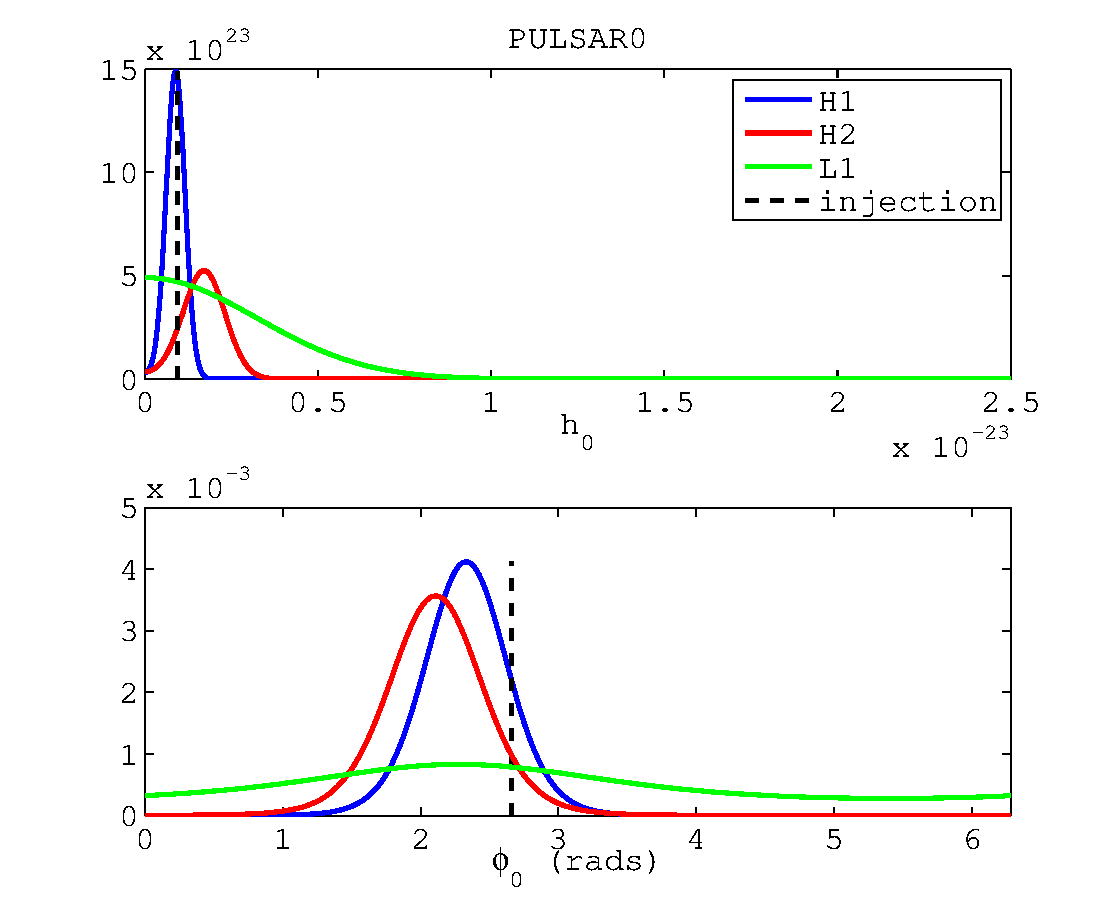
\includegraphics[width=0.33\textwidth]{figs/S3PULSAR0} &
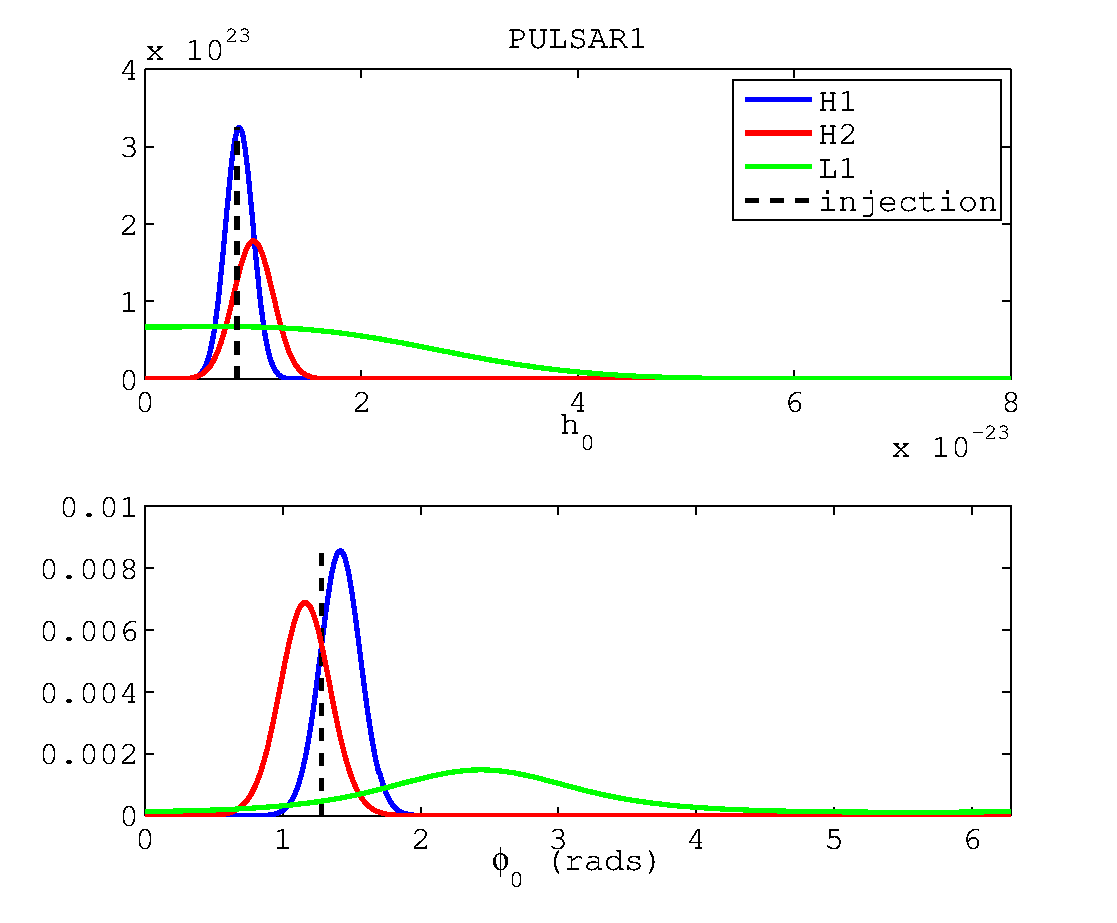
\includegraphics[width=0.33\textwidth]{figs/S3PULSAR1} &
\includegraphics[width=0.33\textwidth]{figs/S3PULSAR2} \\
\includegraphics[width=0.33\textwidth]{figs/S3PULSAR3} &
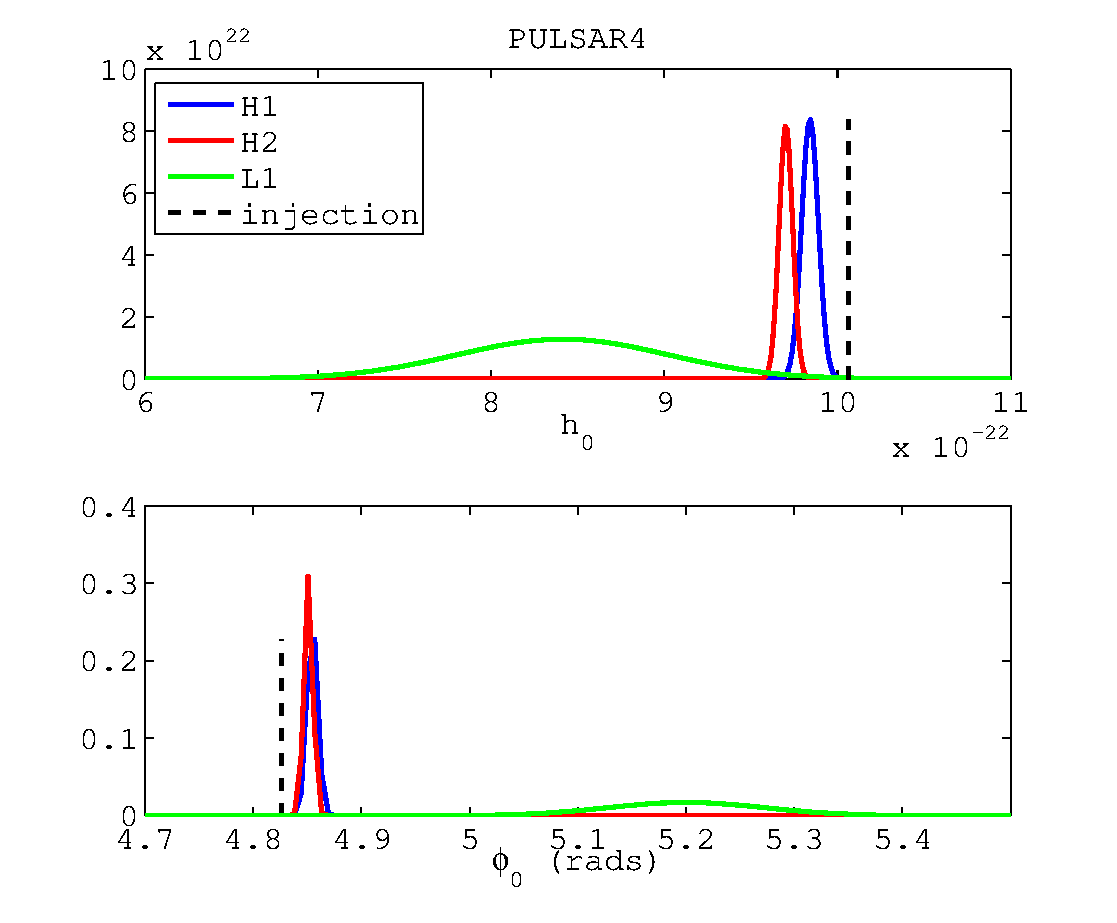
\includegraphics[width=0.33\textwidth]{figs/S3PULSAR4} &
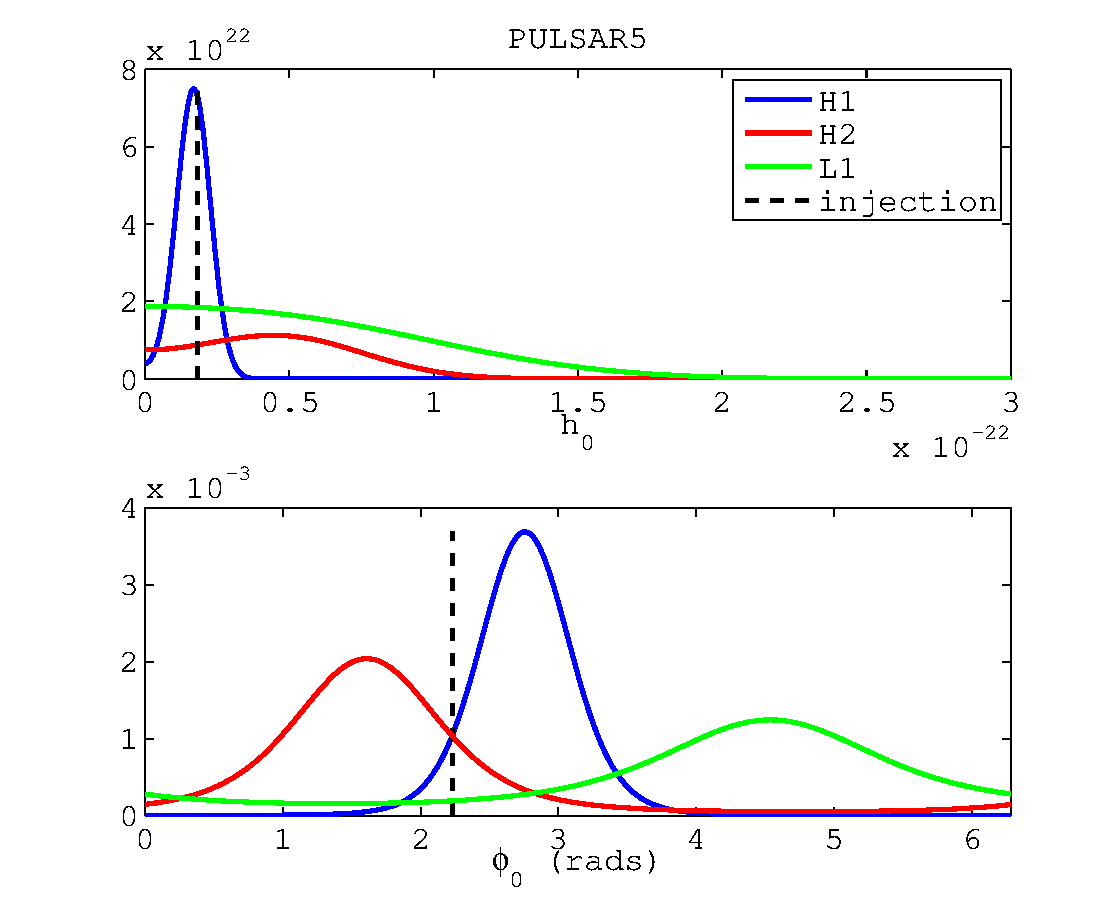
\includegraphics[width=0.33\textwidth]{figs/S3PULSAR5} \\
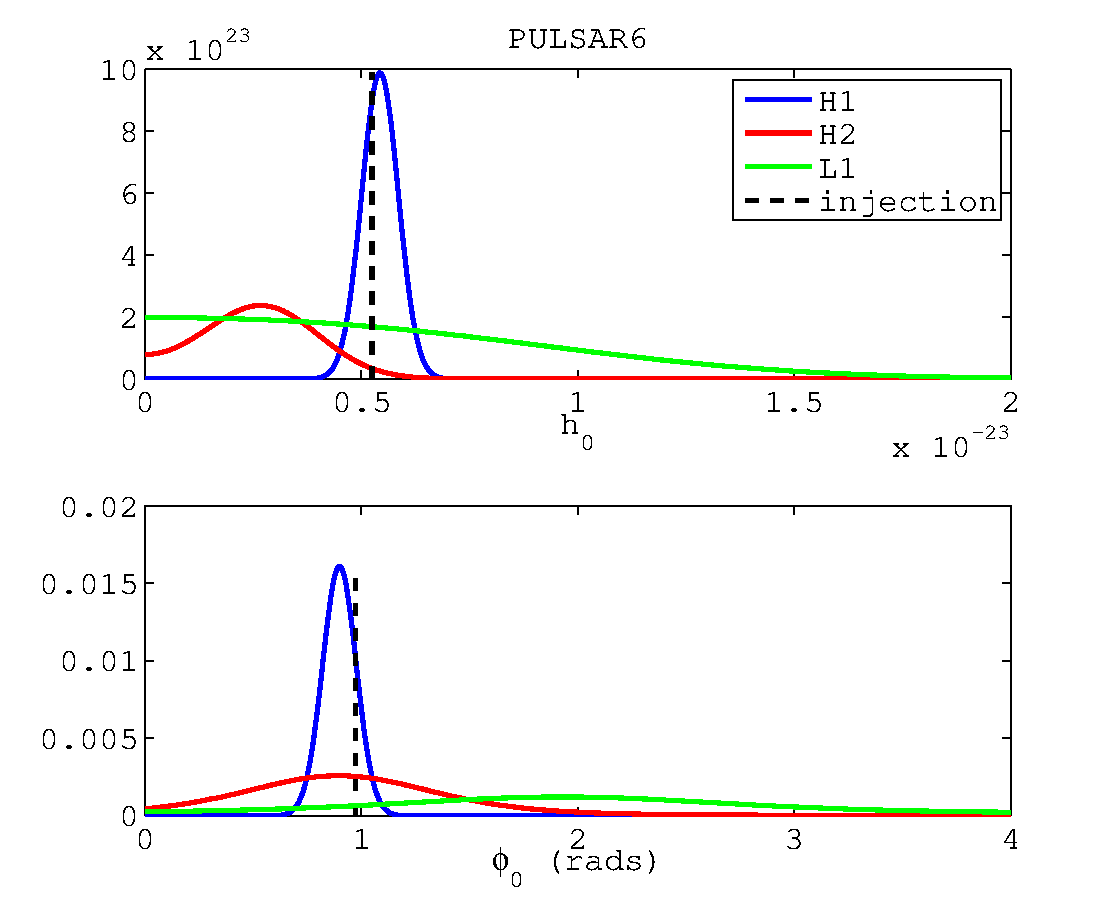
\includegraphics[width=0.33\textwidth]{figs/S3PULSAR6} &
\includegraphics[width=0.33\textwidth]{figs/S3PULSAR7} &
\includegraphics[width=0.33\textwidth]{figs/S3PULSAR8} \\
& \includegraphics[width=0.33\textwidth]{figs/S3PULSAR9} & \\
\end{tabular}
\caption{The pdfs of $h_0$ and $\phi_0$ for 10 injections into the LIGO detectors during
S3.}\label{S3PulsarInj}
\end{figure}

The pdfs in figure~\ref{S3PulsarInj} are not quite the true posteriors that were extracted, but
have been corrected for some calibration differences and injection errors. The $h_0$ pdfs have been
multiplied by a factor related to the difference in the detector actuation function amplitudes
between those used to calculate the injection amplitudes and those used to calculate the final
calibration response function. The ratio of these actuation amplitudes is shown in
figure~\ref{S3ActuationRatio}.
\begin{figure}[!htbp]
\begin{center}
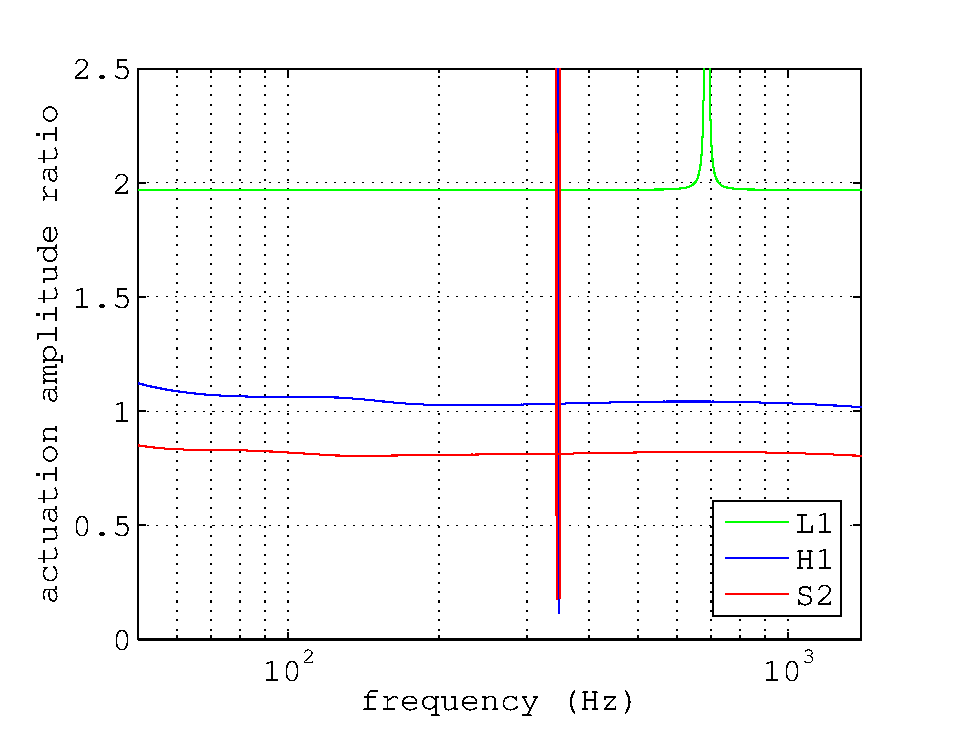
\includegraphics[width=0.6\textwidth]{figs/S3ActuationRatio}\caption[The ratio of the actuation
function amplitudes for the LIGO interferometers.]{The ratio of the actuation function amplitudes
for the LIGO interferometers between that measured for the S3 calibration and that measured prior to
S3 during the E10 engineering run.}\label{S3ActuationRatio}
\end{center}
\end{figure}
For the H1 and H2 interferometers the amplitudes are similar with ratios of approximately 1.0 and
0.8 respectively. For the L1 interferometer there is almost a factor of two difference. In reality
these factors might not quite reflect the true error between the injection amplitudes and those
extracted, as the extracted values actually use the full response function to calibrate the
amplitude, but they do provide an estimate. The variations from the true injected amplitude,
after the above corrections, could also be due to systematic uncertainties in the calibration (a
method of marginalising over these is discussed in \S\ref{MargErrs}), as it can be seen for the
stronger injections that the peak value of $h_0$ for H1 is systematically higher than H2. For L1
there seem to be large uncertainties which cause the pdfs to wander about the true value. The two
other main anomalies are in the amplitudes of P\textsc{ulsar}7 and P\textsc{ulsar}0 in H2.
P\textsc{ulsar}7 appears to be missing from H2, which has been tracked down to the fact that its
amplitude was accidentally set at 1/60 of the supposed injection value. P\textsc{ulsar}0 appears
slightly larger in H1 than H2 (at odds with the general systematic showing the opposite), which is
due to it being injected with an amplitude $\sim 1.6$ larger than expected.

The phases have also been corrected due to an error included during their injection. For the
injections the true values of $\phi_0$ need to be corrected for the actuation phase $\phi_{\rm
act}$. This additional phase was added with the wrong sign leading to the extracted phase being
$\sim 2\phi_{\rm act}$ away from the true value of $\phi_0$. Again there was slight difference
between the actuation phase used for the injection and that used for the calibration it was
extracted with, so the true correction required the subtraction of both actuation phases (although
they were very similar).

After the introduction of these corrections it can be seen that the phases agree with each other to
within a few degrees. This provides some evidence that there is phase coherence between the
detectors and that a joint analysis, combining the data from the detectors, would be possible.
Unfortunately, as the corrections to the phase and amplitudes were included after the fitting
procedure, the joint analysis could not be used on the injections as in \cite{Abbott:2005}.

The \geo injection has been analysed in \cite{Dupuis:2004}. It was injected into the instrument in
a different way to the LIGO injections as described in Weiland {\it et al.} (2004)
\cite{Weiland:2004}. As described in \cite{Dupuis:2004} the phase and amplitude of this signal in
\geo were significantly off their true values due to pickup between the injection hardware and the
interferometer \gw channel.

\subsection{S4 injections}\label{S4injections}
For S4 the 10 initial injections used in S3 were again used to create artificial signals in the LIGO
interferometers. Their amplitudes were adjusted to give approximately the same $S/N$ as for S3, but
taking into account the better sensitivity during this run. For all but P\textsc{ulsar}9 the $h_0$
values were reduced by a half, with P\textsc{ulsar}9 being so strong that its amplitude was
reduced by a factor of 20. The phases for all the injections are also shifted by $\pi$\,radians with
respect to those given in table~\ref{S3InjectionParams}. These signals were injected for the second
half of the run from $8^{\rm th}$ March 2005 onwards. The updated $h_0$ values are shown in
table~\ref{S4InjectionParams}. There were also an additional two signals, simulated to be from
pulsars in binary systems, injected for the last day of the run. The binary pulsar injections
allowed the testing of the binary timing code described in Chapter~2 as the injection code and
extraction code were written independently. The binary injection signal (P\textsc{ulsar}10 and 11)
parameters were taken from P\textsc{ulsar}3 and 8 respectively, with the frequencies changed and
amplitudes increased to make sure they were visible over the short injection time. The frequency,
amplitude and binary system parameters are shown in table~\ref{S4BinInjectionParams}. The binary
system parameters were chosen to have one in a relatively eccentric orbit and one in a circular
orbit with fairly short periods, so that they would have completed or nearly completed at least one
full orbit during the injection. The $T_0$ values are given in the pulsar rest frame\footnote{This
is a difference between the code used to create the signals which took in values of $T_0$ in the SSB
frame and then corrected to the pulsar rest frame, and the code used to extract them which follows
the \tempo convention of defining all epochs in the pulsar rest frame.}.
\begin{table}[!htbp]
\caption{\label{S4InjectionParams} The parameter values for the S4 pulsar hardware injections.}
\begin{center}
\begin{tabular}{l | c c c c c}
P\textsc{ulsar} & 0 & 1 & 2 & 3 & 4 \\
\hline
\footnotesize{$h_0$} & \footnotesize{$4.69\ee{-25}$} & \footnotesize{$4.25\ee{-24}$} &
\footnotesize{$7.81\ee{-24}$} & \footnotesize{$3.08\ee{-23}$} & \footnotesize{$5.03\ee{-22}$} \\
\hline
P\textsc{ulsar} & 5 & 6 & 7 & 8 & 9 \\
\hline
\footnotesize{$h_0$} & \footnotesize{$9.17\ee{-24}$} & \footnotesize{$2.62\ee{-24}$} &
\footnotesize{$1.40\ee{-23}$} & \footnotesize{$3.01\ee{-23}$} & \footnotesize{$8.06\ee{-24}$} \\
\end{tabular}
\end{center}
\end{table}
\begin{table}[!htbp]
\caption{\label{S4BinInjectionParams} The parameter values for the S4 binary pulsar hardware
injections.}
\begin{center}
\begin{tabular}{c | c c c c}
P\textsc{ulsar} & $\nu_{\rm gw}$ (Hz) & $h_0$ & $T_0$ (MJD in GPS) & $P_b$ (days) \\
\hline
\footnotesize{10} & \footnotesize{250.6} & \footnotesize{$1.23\ee{-22}$} &
\footnotesize{51749.71156482407} & \footnotesize{1.35405939} \\
\footnotesize{11} & \footnotesize{188.0} & \footnotesize{$4.93\ee{-22}$} &
\footnotesize{52812.92041175901} & \footnotesize{0.31963390} \\
\hline
 & $e$ & $\omega_0$ (degs) & $a\sin{i}$ (secs) \\
\hline
\footnotesize{10} & \footnotesize{0.0} & \footnotesize{0.0} & \footnotesize{1.65284} \\
\footnotesize{11} & \footnotesize{0.180567} & \footnotesize{322.571} & \footnotesize{2.7564} \\
\end{tabular}
\end{center}
\end{table}

These signals were again extracted using the analysis techniques from Chapter~2. For the binary
system injections the BT model was used, although as no relativistic parameters were included any
of the models could have been used. Figure~\ref{S4PulsarInj} shows the extracted pdfs of $h_0$ and
$\phi_0$ for the 10 isolated pulsar injections, where again $\iota$ and $\psi$ were held fixed at
their known values.
\begin{figure}[!htbp]
\begin{tabular}{l l l}
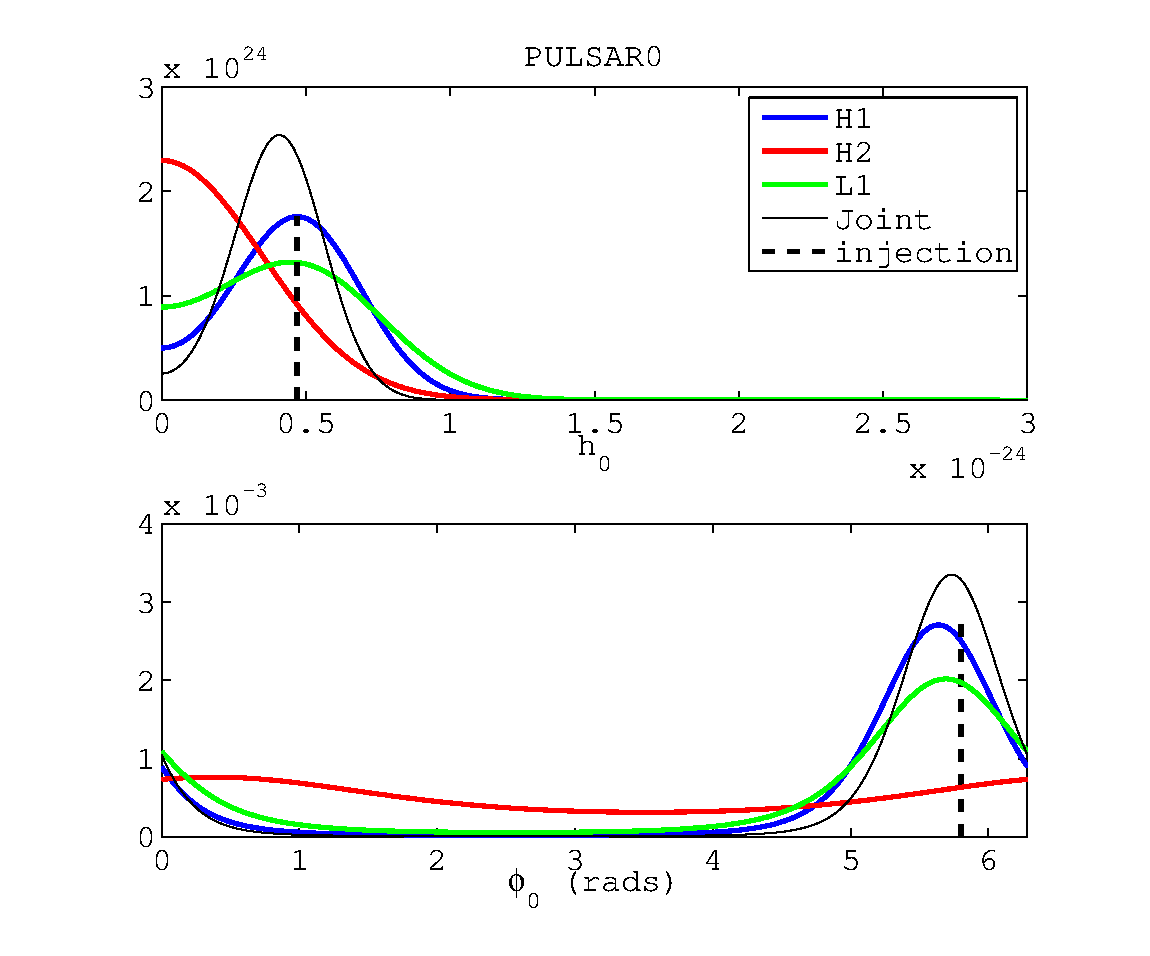
\includegraphics[width=0.33\textwidth]{figs/S4PULSAR0} &
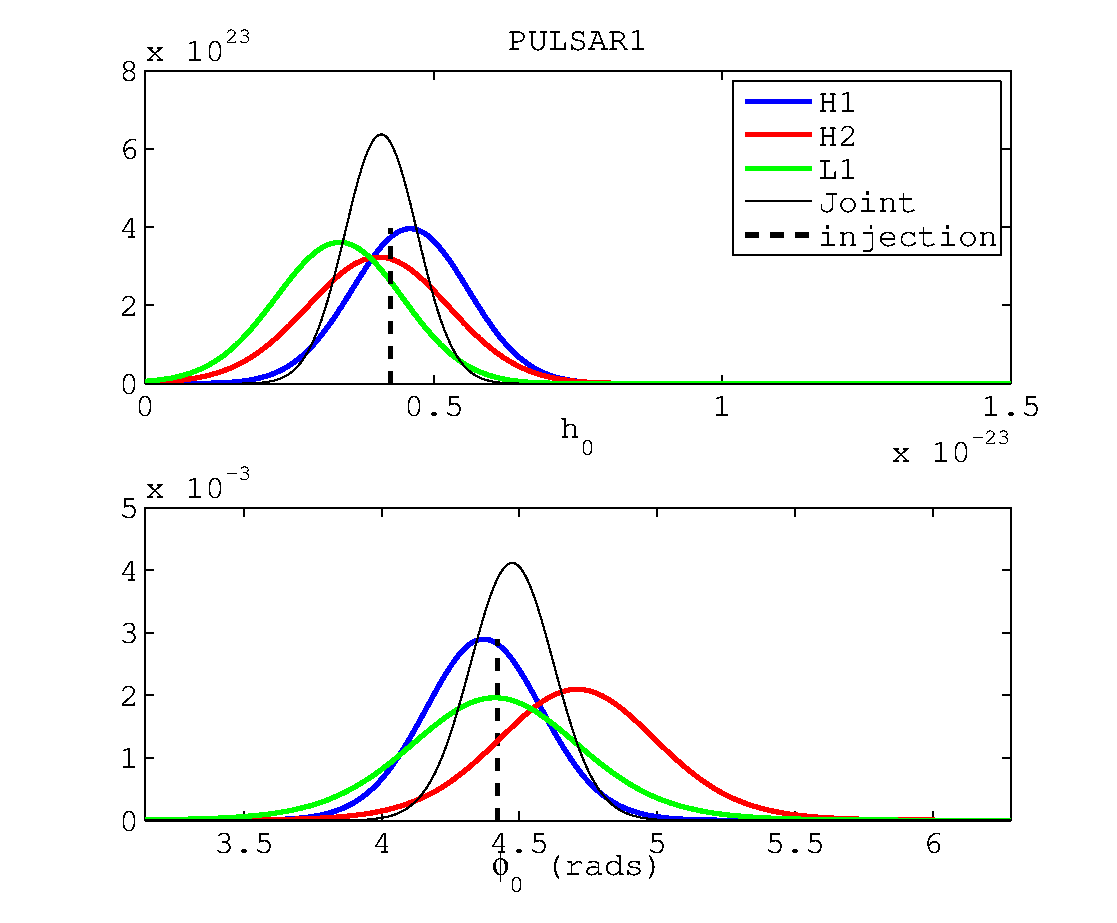
\includegraphics[width=0.33\textwidth]{figs/S4PULSAR1} &
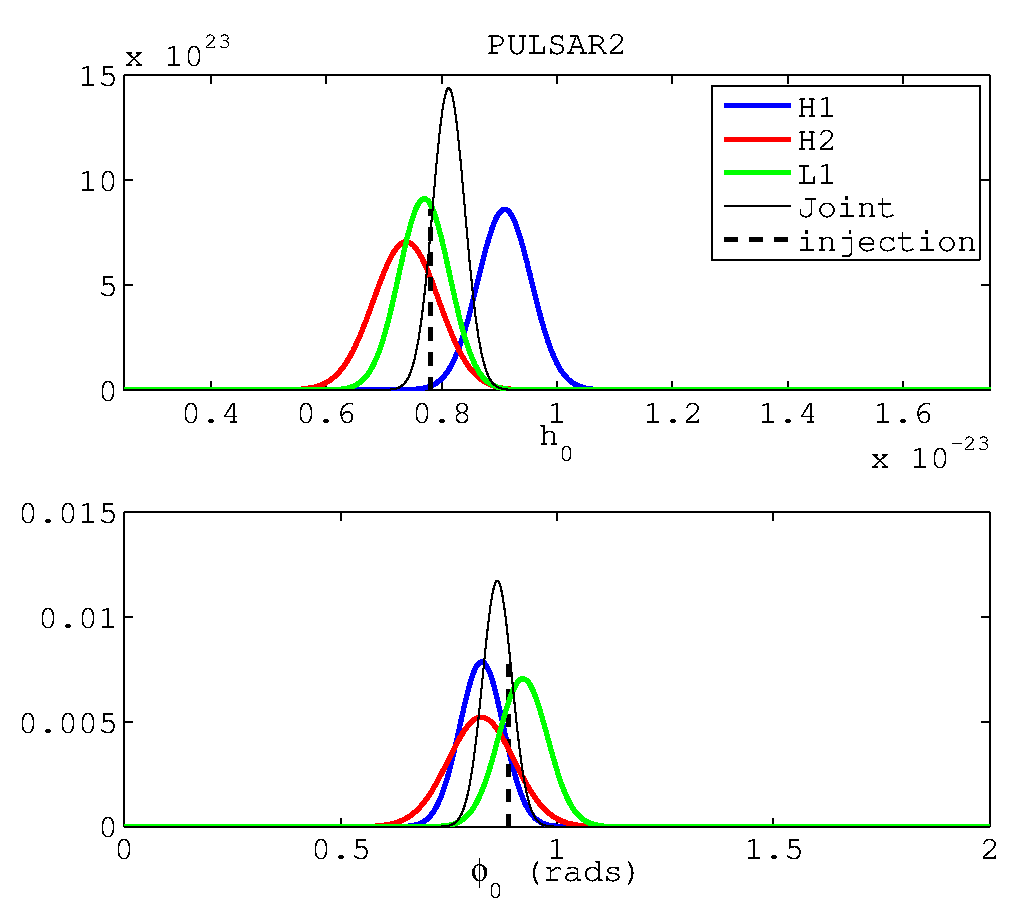
\includegraphics[width=0.33\textwidth]{figs/S4PULSAR2} \\
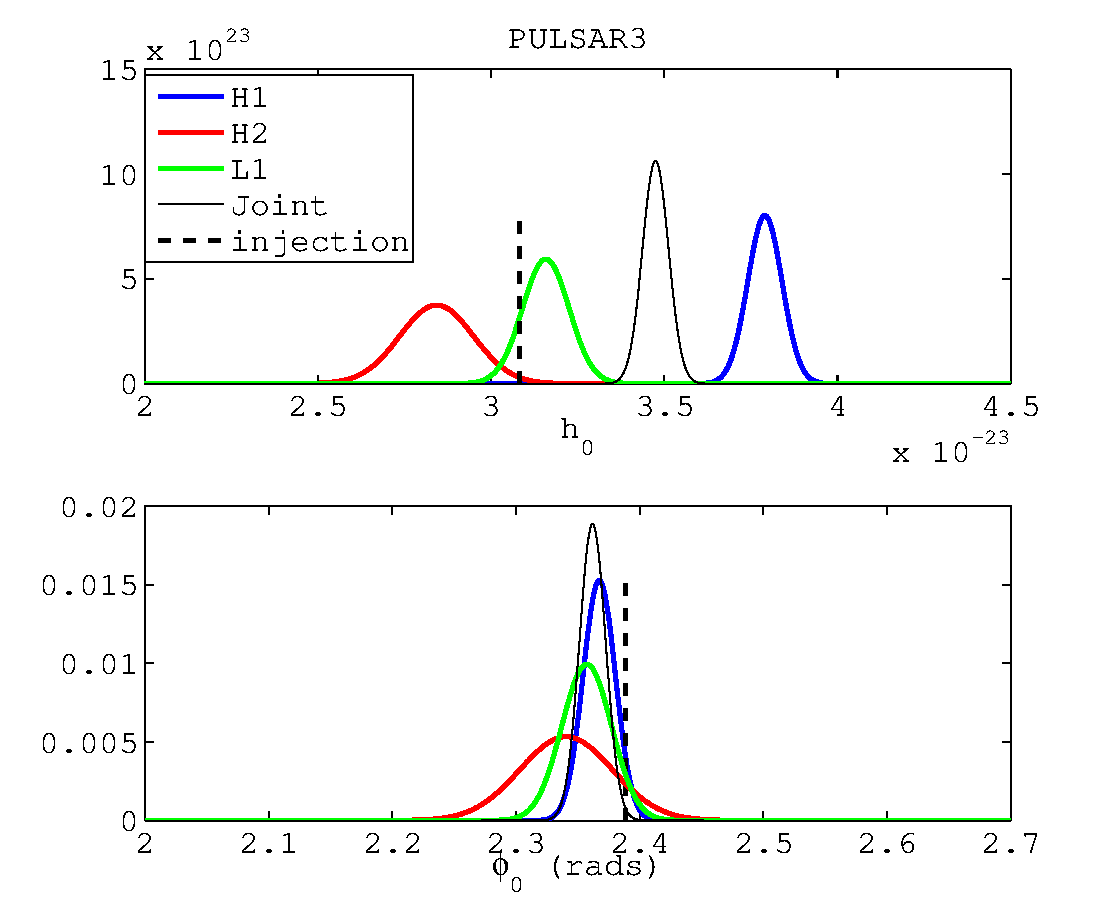
\includegraphics[width=0.33\textwidth]{figs/S4PULSAR3} &
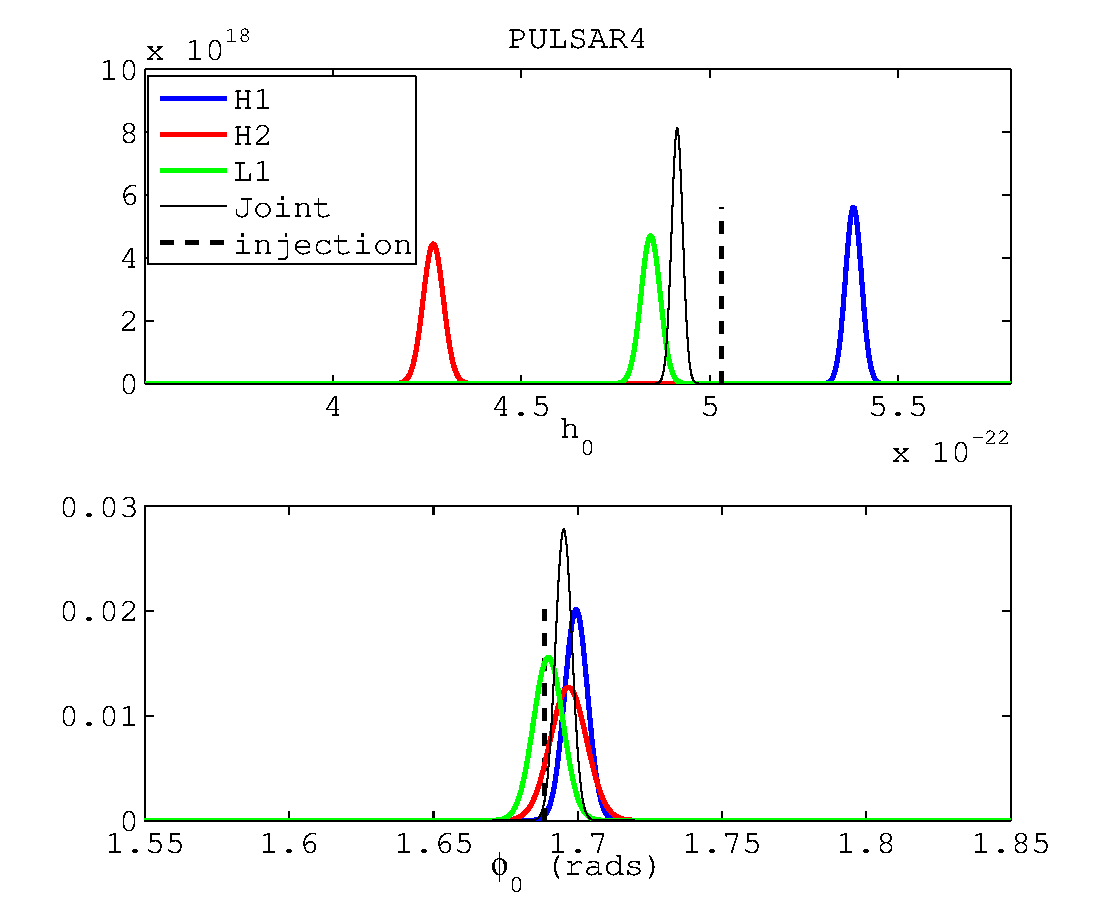
\includegraphics[width=0.33\textwidth]{figs/S4PULSAR4} &
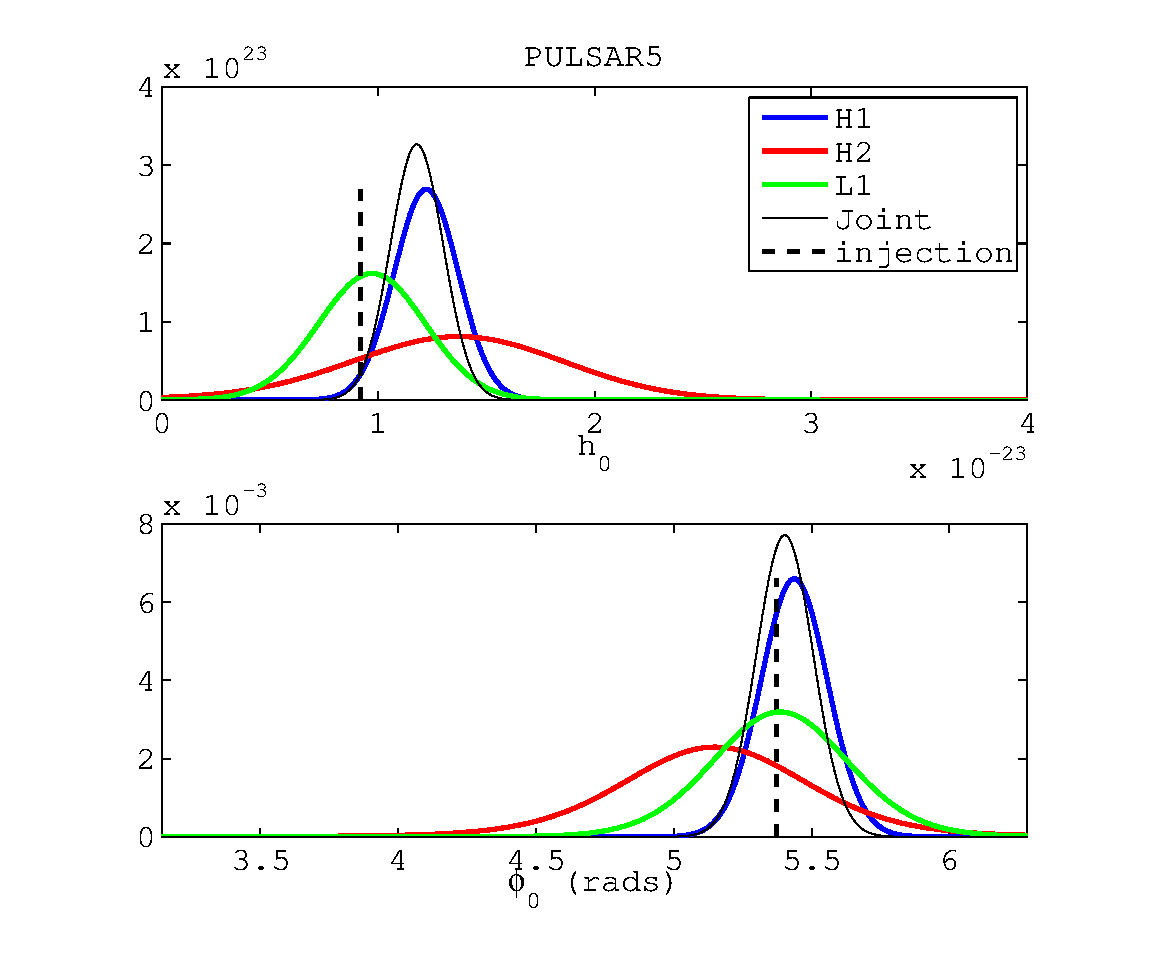
\includegraphics[width=0.33\textwidth]{figs/S4PULSAR5} \\
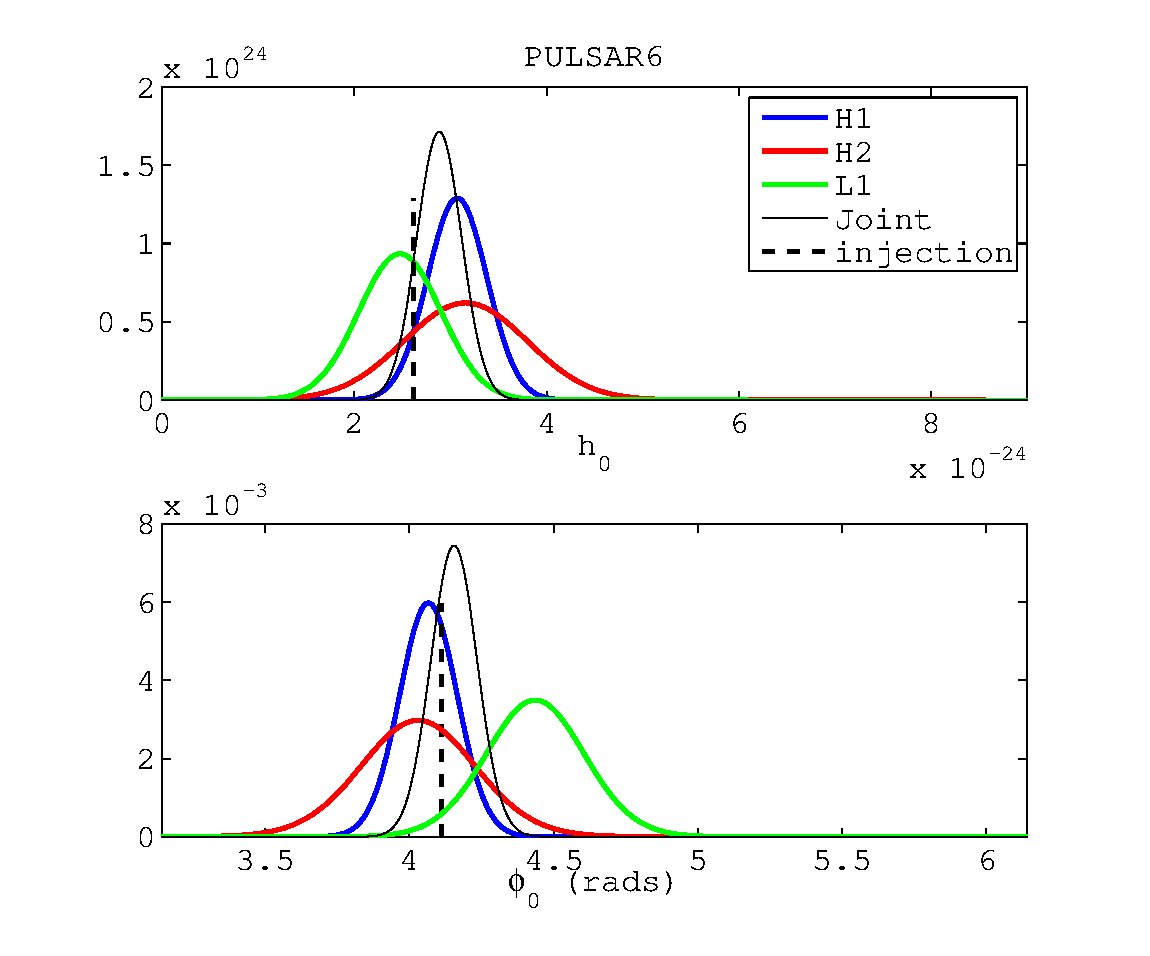
\includegraphics[width=0.33\textwidth]{figs/S4PULSAR6} &
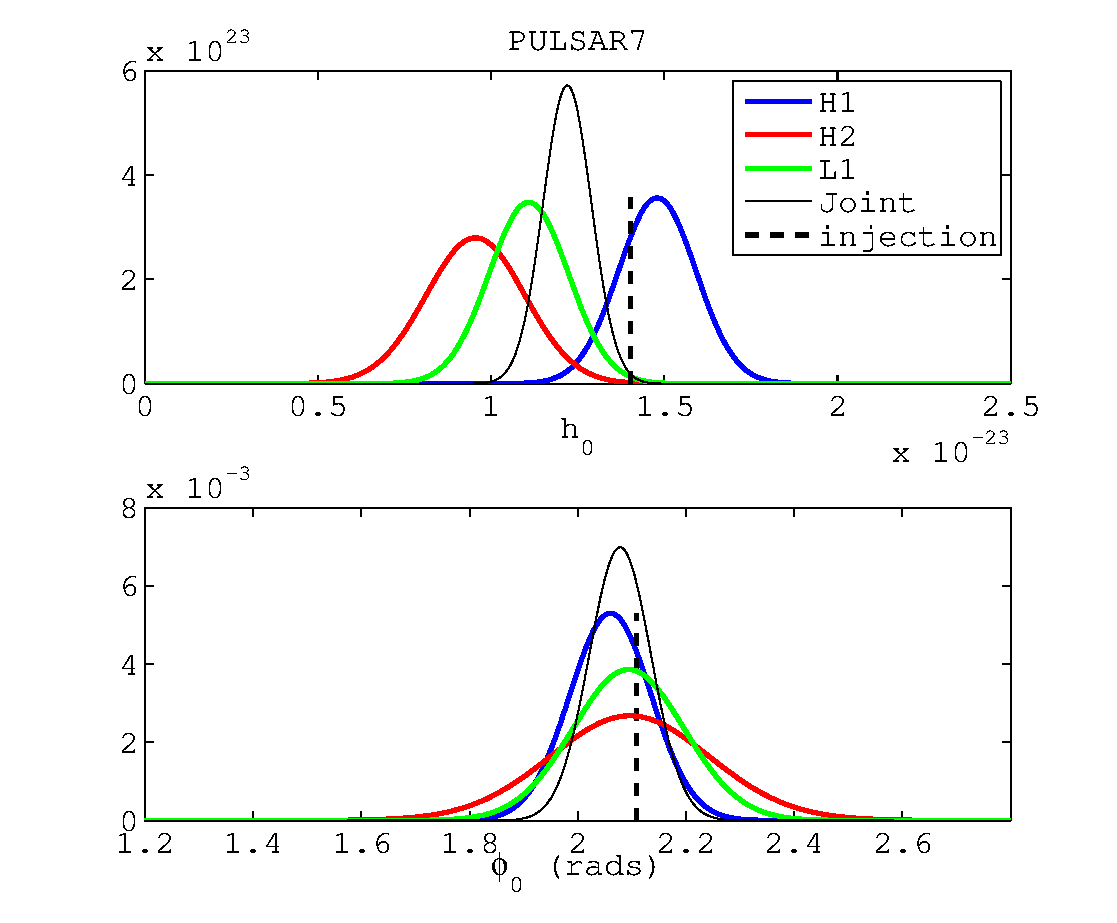
\includegraphics[width=0.33\textwidth]{figs/S4PULSAR7} &
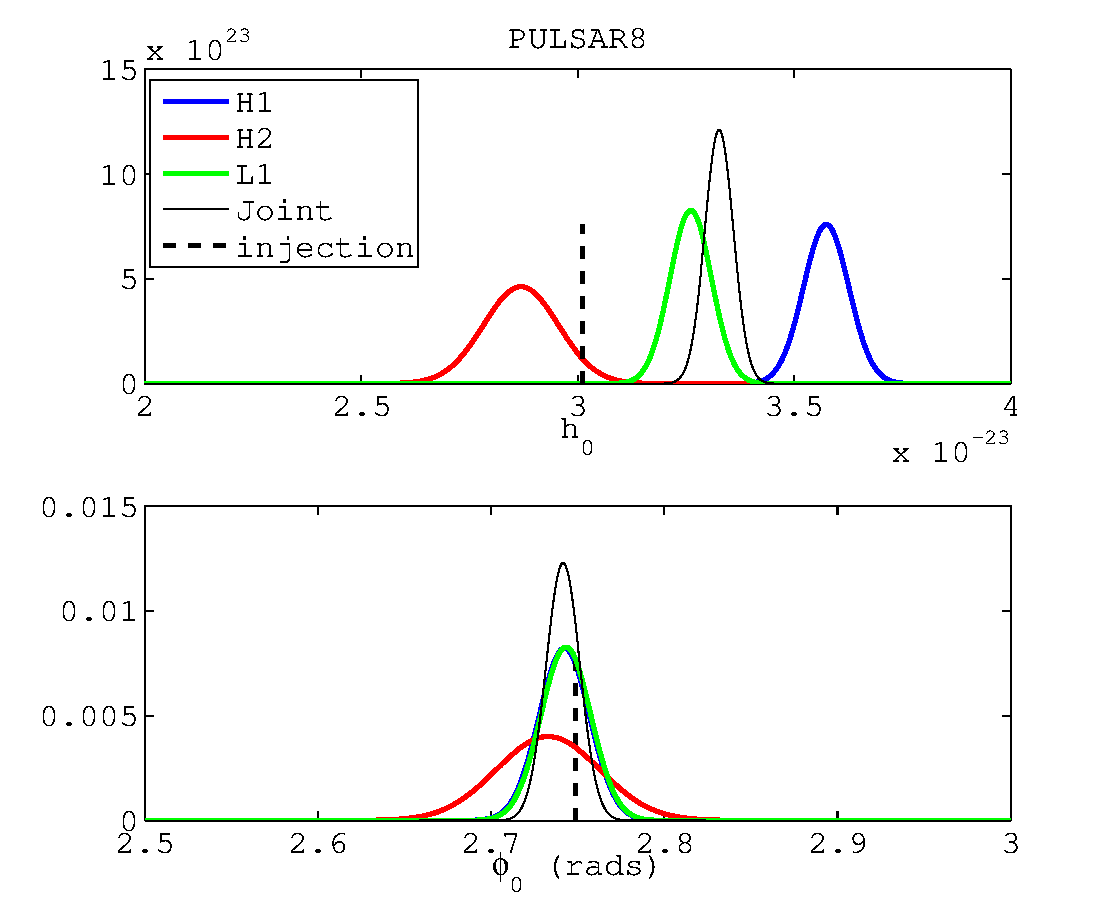
\includegraphics[width=0.33\textwidth]{figs/S4PULSAR8} \\
 & 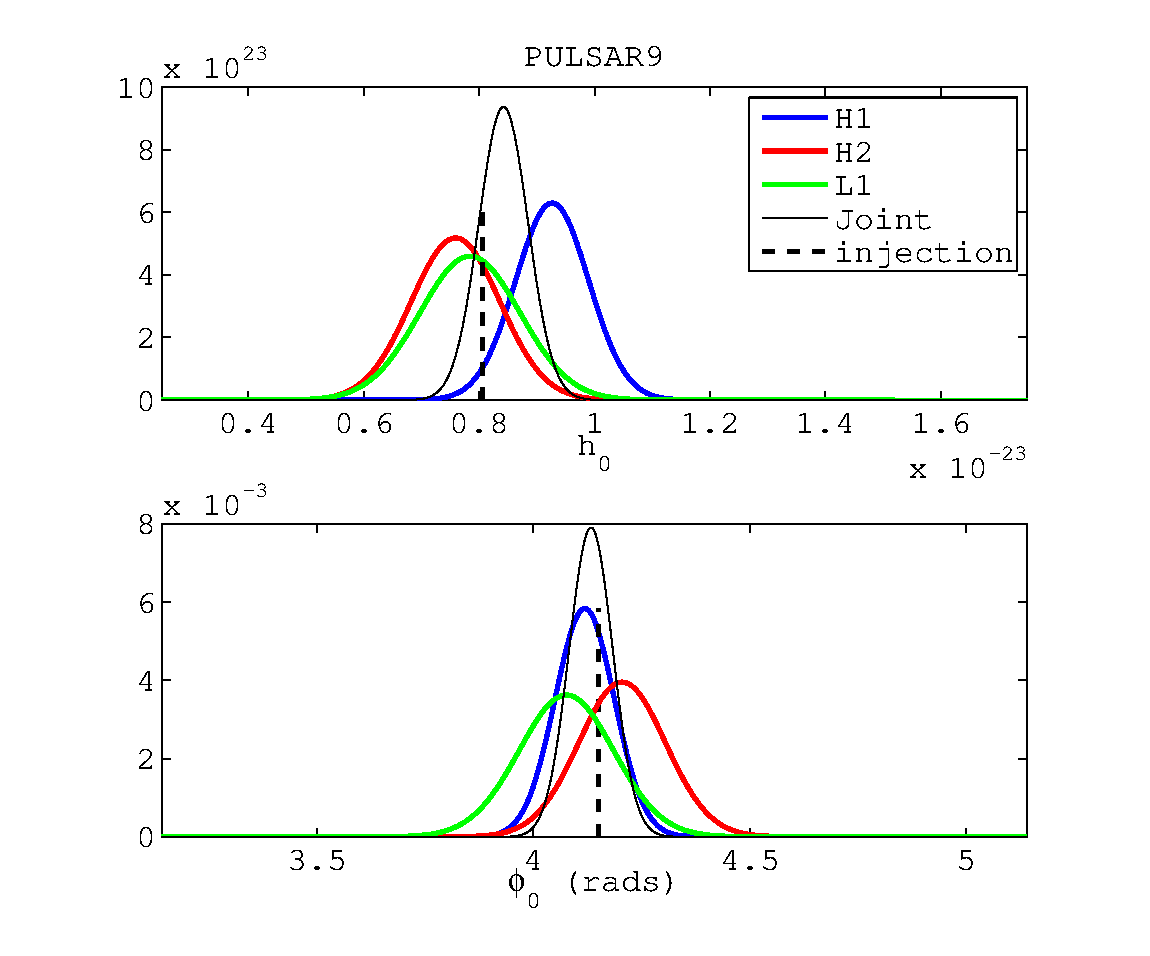
\includegraphics[width=0.33\textwidth]{figs/S4PULSAR9} & \\
\end{tabular}
\caption{The pdfs of $h_0$ and $\phi_0$ for 10 isolated pulsar injections into the LIGO detectors
during S4.}\label{S4PulsarInj}
\end{figure}
Unlike the S3 injection pdfs in figure~\ref{S3PulsarInj} there have been no amplitude corrections
applied to the S4 pdfs, because the calibrations used to calculate the injections and extract the
injections are very similar. 
%The calibration data which has been used has a known error in that the
%phases of H1 and H2 are offset by $\pi$\,radians. As the final, corrected, calibrations were not
%available at the time of writing we have adjusted for this phase error by multiplying the $B_k$s
%by $-1$ i.e. adjusting the phase by $\pi$\,rads. This means the pdfs should show exactly what was
%injected. 
Due to the phase consistency between the detectors the joint likelihood, using all three detectors,
have also been calculated. In general the values of $h_0$ are well matched with the injection
values. Again there are possible systematics which could affect the position of the pdfs. For S4 the
actuation functions used to calculate the injection amplitudes and those used to calculate the final
response function are much more similar than those for S3, with a ratio close to unity. The
actuation phases are also very closely matched.

Figure~\ref{S4BinPulsarInj} shows the pdfs for the two binary system pulsar injections.
\begin{figure}[!htbp]
\begin{longtable}{c c}
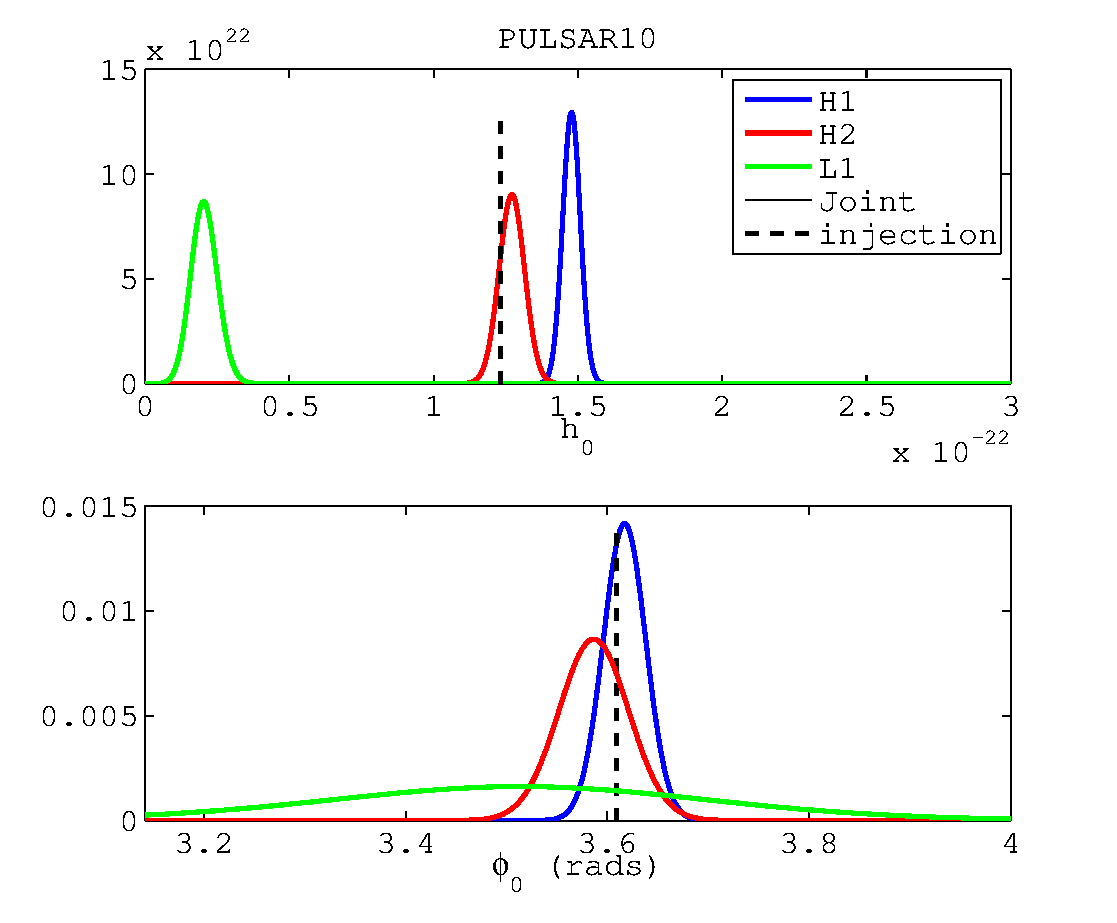
\includegraphics[width=0.33\textwidth]{figs/S4PULSAR10} &
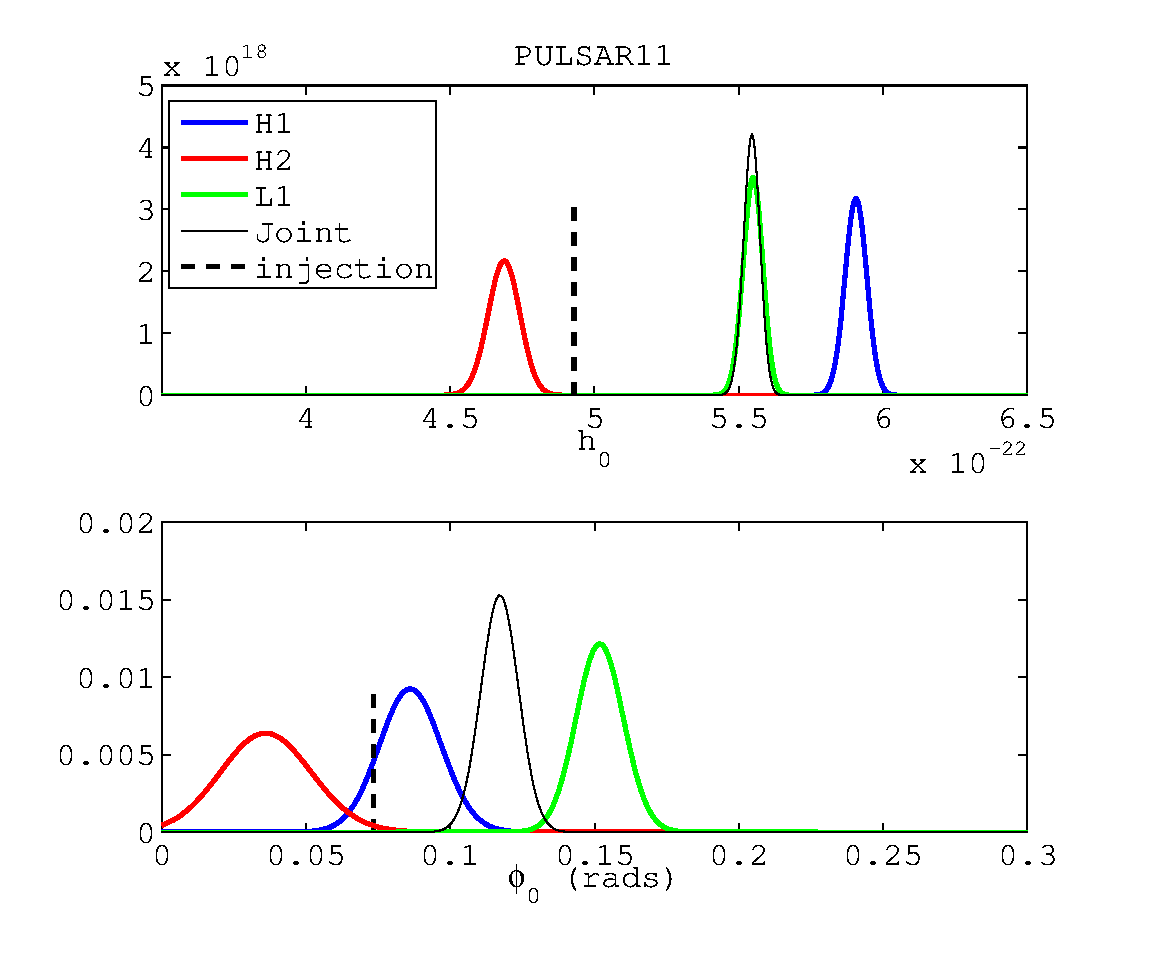
\includegraphics[width=0.33\textwidth]{figs/S4PULSAR11} \\
\end{longtable}
\caption{The pdfs of $h_0$ and $\phi_0$ for the 2 binary pulsar injections into the LIGO
detectors during S4.}\label{S4BinPulsarInj}
\end{figure}
These show similar matches to their injected values as the isolated pulsars. This is a good
confirmation that the binary timing code can track the phase well and has no sign errors (assuming
the independent injection code also does not contain the same sign errors). Here the main apparent
error is the amplitude of P\textsc{ulsar}10 in L1, which appears a factor of $\sim 4$ lower than it
should. At present the source of this error is unknown, although as the amplitude for
P\textsc{ulsar}10 was derived from that of P\textsc{ulsar}3 multiplied by four, it could just be
that this multiplication was left out.

% These results will be reproduced with the final calibration when it is available.

\section{Pulsar selection}
The first criterion for selecting known pulsars to be included in this search was their frequency,
the limiting factor being the low frequency noise floor of the detector. Below about 50\,Hz the
noise floor of the LIGO detectors increases rapidly making searches below this frequency a poor
prospect. This is shown as a law of diminishing returns by equation~\ref{Pulsarh0} where the pulsar
amplitude goes as $\nu^2$, but the noise floor rises dramatically at low frequencies, so in
general pulsar \gw amplitudes will be smaller in a frequency range that has a far worse detector
sensitivity. The choice of a 50\,Hz \gw frequency cut-off (pulsar spin frequency of 25\,Hz) is still
somewhat arbitrary, but it also in some ways represents the split between the population of fast
(millisecond/recycled and young) pulsars and slow pulsars.

The first stage of the selection process involved using the ATNF online pulsar catalogue
\cite{ATNF} (described in Manchester {\it et al.}, 2005 \cite{Manchester:2005}) which provides a
list of pulsars and their parameters. As stated in Chapter~2 this catalogue shows that there are
currently 150 pulsars with spin frequencies $> 25$\,Hz. The accuracy of these parameters varies for
each pulsar, and is dependent on several factors such as when it was discovered, how often it is
monitored or even whether the catalogue has been recently updated with current best fits. The
accuracy of the parameters is important in our search to make sure parameter errors do not lead to
unacceptable phase errors in the heterodyne. Also important is the epoch of the parameters as more
recent measurement will better reflect to current state of the pulsar. Such considerations are not a
problem for the Crab pulsar as it is monitored on a very regular basis, so parameters are
continuously updated \cite{CrabEphemeris}. Working closely with Andrew Lyne and Michael Kramer from
Jodrell Bank Observatory we were supplied with up-to-date parameter information on as many pulsars
as possible. They provided us with parameters for 75 pulsars for which recent timing data from
around the period of the S3 run was available. For many of the other pulsars recent timing was
either not present or unobtainable. For all pulsars the parameters were estimated using the whole
set of data available. For pulsars where their timing straddled S3, the frequency (and occasionally
frequency derivative) parameters were then re-estimated over that period with the other
parameters held fixed at their previously calculated values. When \tempo fits a parameter it will
calculate the associated uncertainty on that parameter (ostensibly a $1\sigma$ error, although in
reality it is more commonly assumed to be $\sim \frac{1}{2}\sigma$), but no uncertainty will be
produced if the parameter is fixed. This meant that if the pulsar parameters were re-fitted over S3
any uncertainty associated with the fixed parameters would be folded into the estimate of the freely
varying frequency parameters (including effects of timing noise for example). Since we are not
terribly concerned with how good the fits are, but only whether the best parameters allow us to
model the phase accurately (i.e. can they be used to unwind what \tempo did to produce them) the
parameter values should be exactly what we need for S3.

The final number of pulsars used for the S3 and S4 analyses is 93. The extra pulsars had their
parameters taken from the most recent values on the ATNF catalogue, except PSR\,J0537-6910 for which
parameters were taken from Marshall {\it et al.} (2004) \cite{Marshall:2004} and the Crab pulsar
where parameters were taken from the monthly ephemeris \cite{CrabEphemeris}. This still left 57
pulsars out of the analysis for which a judgement was made that the parameters were not defined
accurately enough for our needs. This judgement call was easy for many of the newly discovered
pulsars (for example the 21 newly discovered milliseconds pulsars in the Terzan 5 globular cluster
in Ransom {\it et al.}, 2005 \cite{Ransom:2005}) where simply not enough observations have been
collected to give good parameter estimates.
 
\subsection{Parameter checking}
For pulsars where the radio parameter estimation was not performed over the epoch of S3, as timing
was unavailable, it is worth checking whether the parameter errors could be enough to cause serious
uncertainties in the heterodyne phase. For all pulsars this is an important consideration for the S4
run as no new timing has yet been obtained for this period. For all pulsars there are positional
errors, which could affect the solar system barycentring time delay, and there are frequency and
frequency derivative errors, all of which can affect the phase accuracy. For pulsars in binary
systems there are errors associated with all the binary orbital parameters, which can again affect
the phase through barycentring time delay errors. These errors are not necessarily uncorrelated
though, for example the error on frequency could affect the accuracy of the first frequency
derivative, and the binary time of periastron and longitude of periastron are highly correlated.

It is useful to see what effect these errors have on the phase over the course of S3 and S4, by
propagating them over the period of the runs. We can just add/subtract errors from the best fit
values of all the parameters and work out the combination which gives a maximum phase deviation from
that found using the best fit values. Due to the correlations between certain parameters this will
give a conservative limit on the maximum phase error. \tempo can be used to produce a covariance
matrix for each of these parameters, which would take into account the correlations, but
unfortunately this was not done for the parameters produced for S3.

When applying this we chose a criterion that any phase error $> 30^{\circ}$ is unacceptable. This
criterion was somewhat arbitrary, but was thought to be a reasonable compromise as it is small
enough not cause a too much decoherence of a possible signal and large enough to avoid excluding too
many pulsars. Applying this to S3 it is seen that 13 pulsars lie above this limit\footnote{for
tables of errors see \url{http://www.astro.gla.ac.uk/~matthew/analyses/ParamErrors.htm}.}. Eight of
these are in binary systems: PSRs\,J0024-7204H, J0407+1607, J0437-4715, J1420-5625, J1518+0205B,
J1709+2313, J1740-5340 and J1918-0642, and five are isolated: PSRs\,J0030+0451, J0537-6910,
J1721-2457, J1730-2304 and J1910-5959B. For five of the binary systems it is the $T_0$ and
$\omega_0$ parameters which contribute most to the phase error. However, it also the case that these
pulsars are in very low eccentricity (highly circular) orbits, thus meaning the errors on the $T_0$
and $\omega_0$ parameters are intrinsically hard to measure and will most likely be far smaller than
the quoted value. For these pulsars we can recalculate the phase error with the errors on $T_0$ and
$\omega_0$ set to zero and we find that for four of them (PSRs\,J0024-7204H, J0407+1607, J1420-5625,
J1709+2313) the error now falls below our limit of $30^{\circ}$. For the other pulsars it is the
error on the frequency and/or position parameters, or in a couple of the binary cases the period
error, which contribute most to the phase error.

Applying this to S4, using the above phase error limit, we actually have one pulsar
(PSR\,J1910-5959B) fall back below the limit leaving 12 pulsars above it. This is due to the
frequency parameter errors contributing most to the phase error for this pulsar and therefore with
the shorter timespan of S4 not so much phase error could accumulate. If new parameter estimations
over the period of S4 are made then these will be used in the future. 

This is not to say that for the pulsars where the phase error is possibly large it will be, as
these are the worst case values. Therefore, results for these pulsars will still be given, but will
retain a caveat that they could be unreliable due to possible phase errors. This could mean that
for pulsars where the maximum phase error $\Delta\phi_{\rm max}$ is $< 90^{\circ}$ the upper limits
may need scaling by $\sim 1/\cos{\Delta\phi_{\rm max}}$, and if $\Delta\phi_{\rm max}$ is $\ge
90^{\circ}$ the results will have to be discarded. With our limit of $30^{\circ}$ this would
lead to a scaling in amplitude of $\sim 15\%$. In general results just reflect the noise floor
anyway, although it would be wrong to say that an upper limit was for a particular pulsar, rather
than for just a particular area of the noise floor, if it was known that the phase used in the
search was definitely wrong. Here we will give the best fit parameter values the benefit of the
doubt and accept them all as correct, with the above caveat. In the future when we obtain pulsar
timing we will be supplied with the covariance matrix of the parameters, thus allowing us to
calculate phase errors in a far more rigorous and non-conservative way.

\subsection{Timing noise}
Timing noise was described in Chapter~2 with particular focus on the Crab pulsar. For the Crab
pulsar the timing noise can be taken account of via a second heterodyne procedure as its phase
evolution is regularly followed. For other pulsars some way to estimate the effect of timing noise
on its phase is needed that does not rely on continuous observation. One such estimate is the
$\Delta_8$ parameter given by equations~\ref{delta8} and \ref{delta8slope}, which provides a
cumulative phase error by assuming the measured $\ddot{\nu}$ is dominated by timing noise. 
Therefore, this can only really be estimated empirically for pulsars for which a value of the second
frequency derivative has been measured. For other pulsars an estimate can be made using the linear
relation fit between the period derivative $\dot{P}$ and $\Delta_8$ in Arzoumanian {\it et al.}
(1994) \cite{Arzoumanian:1994} as given in equation~\ref{delta8slope}. The values of $\Delta_8$ and
its corresponding cumulative rotational phase error are given in table~\ref{delta8table} and shown
in figure~\ref{delta8figure}.
\begin{figure}[!htbp]
\begin{center}
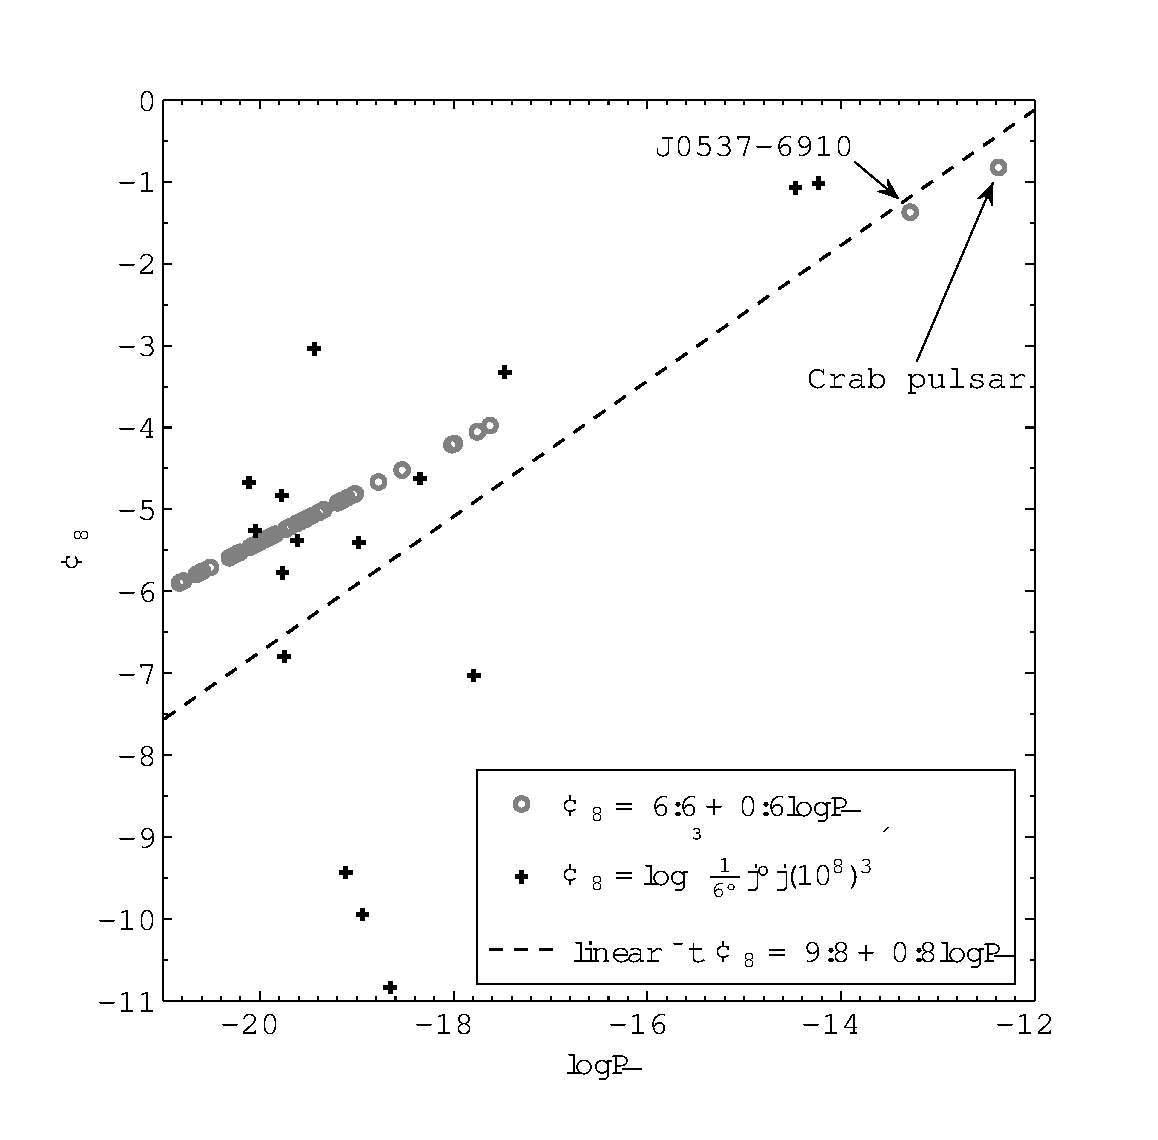
\includegraphics[width=0.6\textwidth]{figs/delta8}
\caption{The values of $\Delta_8$ for our selection of pulsars.}\label{delta8figure}
\end{center}
\end{figure}
Figure~\ref{delta8figure} also shows a linear fit to values for which $\ddot{\nu}$ has been used to
calculate $\Delta_8$ given by $\Delta_8 = 8.9 + 0.8\log{\dot{P}}$. If this fit was to be used
instead of equation~\ref{delta8slope} (which was fitted by eye) it would make little difference for
the majority of pulsars as their $\Delta_8$ values are already small. For the linear fit a value of
the intrinsic spin-down (discussed in more detail in \S\ref{results}) has been used when available
and if positive. For pulsars which were re-timed over the period of S3 timing noise should not be a
problem at all (for the S3 analysis at least) as any timing noise, which usually has variations on
time scales of several month to years, will have been folded into the other parameters.
\input bigtables/delta8.tex

Almost all the timing noise phase errors are small enough to be negligible for our analysis.
Using the same $30^{\circ}$ phase error criterion as with the parameter errors we see that the
estimated timing noise is not negligible for six pulsars: PSRs\,J0534+2200 (Crab pulsar),
J0537-6910, J1748-2446A, J1823-3021A, J1913+1011, and J1952+3252. The $\Delta_8$ values for the Crab
pulsar and PSR\,J0537-6910 have been obtained from the linear relation even though they have very
accurately measured values of $\ddot{\nu}$. This is because for these pulsars timing noise will not
be the dominant component of $\ddot{\nu}$. The value for the Crab pulsar is not important as the
timing noise is taken into account with an extra heterodyne. For the other five pulsars it could be
important, so these results will be flagged as possible problem pulsars. As for the pulsars with
possible parameter errors all the results presented here will give the benefit of the doubt that
timing noise has not had an adverse effect, therefore the results should be treated with caution.

There are pulsars in globular clusters for which there is no $\ddot{\nu}$ and $\dot{P}$ is negative
($\dot{\nu}$ is positive), so no value of $\Delta_8$ can be assigned. For these pulsars the value of
$\dot{\nu}$ (and therefore $\ddot{\nu}$) must be rather small to have been affected by globular
cluster motions (discussed more in \S\ref{results}), so timing noise should be negligible.

\subsection{The data}
The results presented below make use of heterodyned data as described in Chapter~2. For each
science run there were various cuts made in what data was used. The first and most obvious cut was
to use only data taken when the detectors were in lock in so called science mode. This is data
which has been deemed to be of good quality. The science mode segments were obtained using the
LIGOtools \cite{LIGOtools} code {\tt segwizard}. The length of times of these science mode segments
represent the full data set for the runs.

The first cut after this was from dividing the data into the 60 seconds chunks that comprise each
$B_k$ value. This meant that up to 60 seconds could be lost from each locked stretch of data. The
start of each locked stretch would also have, by definition, been preceded by a discontinuity in
the data. Such a discontinuity would cause the filters in our analysis to ring and produce an
apparent glitch in the $B_k$s. This being so the first $B_k$ after the beginning of a lock
stretch was removed in post-processing. 

The heterodyning was performed on large computer clusters where the data was split up between the
available computers. This splitting of data meant that it artificially introduced discontinuities in
the data for each chunk. This would again ring the filters, so the first $B_k$ was always
removed. For the analysis on the LSC computer cluster at
Caltech\footnote{\url{http://ldas-gridmon.ligo.caltech.edu/ganglia}}, with 580 processors, this
meant that almost 10 hours of data was artificially contaminated and removed.
% write a bit about how much data was used /cut out etc
% say about Rejean's KS test
The Bayesian analysis we use makes the assumption of stationarity of the data over a certain length
of time. In the previous analysis of S2 \cite{Abbott:2005} this length of time was fixed at the
fairly arbitrary value of 30 minutes, so the value of $m_j$ in equation~\ref{StudentstLikelihood}
was always 30. This meant that only contiguous 30 minutes segments could be used, again discarding
more data. In our current analysis this 30 minute limit becomes the maximum length of a data
segment, with segments smaller than this now being allowed. A lower limit on segment lengths of
5 minutes was set, as it was felt that very little more information could be added from segments
shorter than this. This allowed the majority of the $B_k$s to contribute to the analysis.

In Dupuis (2004) \cite{Dupuis:2004} a Kolmogorov-Smirnoff test was used to check the validity of the
assumption of stationarity over each 30 minute segment for S3. This generally showed about 20\% of
all segments did not conform to this assumption. Despite this all segments have been included,
because as stated in \S\ref{TimeDomainMethod} the Gaussian distribution is the least informative
distribution and any deviations from it will be incorporated as extra noise.
% show some B_k plots

\section{Results}\label{results}
Here we will present 95\% degree-of-belief upper limits on the amplitude of gravitational waves
($h_0$) emitted from the 93 pulsars as discussed above. The value of $h_0$ is independent of any
assumptions about the neutron star other than it being triaxial and therefore emitting \gws at twice
its rotation frequency. The results will also be presented in terms of the pulsars' equatorial
ellipticity $\varepsilon = (I_{xx} - I_{yy})/I_{zz}$, which under this assumption of triaxiality can
be related to $h_0$ via
\begin{equation}\label{h0epsilon}
\varepsilon = 0.237\left(\frac{h_0}{10^{-24}}\right)\left(\frac{r}{1\,{\rm
kpc}}\right)\left(\frac{1\,{\rm Hz}^2}{\nu^2}\right)\left(\frac{10^{38}\,{\rm kg}\,{\rm
m}^2}{I_{zz}}\right),
\end{equation}
where $I_{zz}$ is the principle moment of inertia, $r$ is the distance to the star and $\nu$ is the
pulsar frequency\footnote{{\it not} the gravitational wave signal frequency.} \cite{Abbott:2005}. To
obtain an upper limit on $\varepsilon$ from that found for $h_0$ the fiducial moment of inertia
value of $I_{zz} = 10^{38}$\,kg\,${\rm m}^2$ is generally used. The validity of this is discussed
later.

The results are also presented in comparative terms as a ratio with the upper limit deduced
from spin-down arguments via equation~\ref{spindownUL}. This makes the assumption that all
rotational energy is lost via \gw emission, which for some cases is known to not be true (see
\S\ref{CrabPulsarResults}). Despite this the spin-down limit is seen as a natural crossing point
after which we can begin to speculate on the nature of the neutron star. The spin-down upper limit
will obviously depend on the rate of spin-down, this value however, can be masked by radial
and transverse motions of the object (see Lyne and Graham-Smith, 1998 \cite{PulsarAstronomy}). The
Shklovskii effect \cite{Shklovskii:1970}, in which the pulsar has a large transverse velocity $v$,
will cause an apparent rate of change in the pulsars period of
\begin{equation}\label{ShklovskiiEffect}
\dot{P}_{\rm S} = \frac{v^2}{rc}P,
\end{equation}
where $r$ is the pulsar's distance. With its $1/r$ scaling this is obviously more prominent for
close by pulsars. In the ATNF catalogue \cite{ATNF} values of the intrinsic period
derivative $\dot{P}_{\rm int} = \dot{P}-\dot{P}_{\rm S}$ can be obtained with this effect corrected
for. This provides an intrinsic spin-down rather than that measured\footnote{Note that the
heterodyne procedure still needs to make use of the measured spin-down rather than the intrinsic
spin-down as these Doppler effects will have the same effect on the gravitational waves.}, and for
cases where it is available this is the value that is used for the spin-down ratio.

Another cause of changes to the observed pulsar $\dot{P}$ is if it is being accelerated in a
gravitational field, like that of a globular cluster. If there is a radial component of the
velocity $v_r$, then the observed value of $\dot{P}=(1+v_r/c)\dot{P}_{\rm int}$ (Phinney, 1993
\cite{Phinney:1993}). These effects can cause pulsars to have apparent spin-ups (seen in quite a
large number of globular cluster pulsars) although are only strong enough to greatly effect pulsars
with intrinsically small period derivatives. There are still many globular clusters for which the
radial accelerations have not been measured, therefore no spin-down upper limit can be set, making
the direct \gw results a unique limit.

\subsection{Marginalising over errors}\label{MargErrs}
\subsubsection{Calibration errors}
When calculating the pdfs for $h_0$ above there was no account taken of the errors/uncertainties in
calibration. In previous work \cite{Abbott:2004, Abbott:2005} these have just been quoted as a
percentage uncertainty in the final result. It is possible to fold the errors into the results,
where it is in fact seen that they make no difference (under the assumption that the error is
additional random noise). Following work done by Romano (2005) \cite{Romano:2005} we can model the
calibration error as a extra parameter $\lambda$ in our likelihood function, so
\begin{equation}
B_k \to \lambda{}B_k, {\rm and~} \sigma_j \to \lambda\sigma_j.
\end{equation}
Applying this to equation~\ref{NoiseIntegral} we get
\begin{equation}
p(\{B_k\}_j|\mathbf{a}, \lambda) \propto \int_0^\infty
\frac{1}{(\lambda\sigma_j)^{2m_j+1}}\exp\left(-\frac{1}{2(\lambda\sigma_j)^2}\sum_{k=1}^{m_j}
|\lambda { } B_k - y_k|^2\right) \rm{d}(\lambda\sigma_j),
\end{equation}
which after integrating leaves
\begin{equation}
p(\{B_k\}_j|\mathbf{a},\lambda) \propto \frac{1}{\lambda^{2m_j}}\bigg(\sum|B_k -
y_k/\lambda|^2\bigg)^{-m_j}.
\end{equation}
If we use a uniform prior distribution for $\lambda$, and give some range for the calibration
uncertainty between $\lambda_{\rm min}$ and $\lambda_{\rm max}$, we can marginalise over it,
\begin{equation}\label{MargCalibUncertEqn}
p(\{B_k\}_j|\mathbf{a}) \propto \int_{\lambda_{\rm min}}^{\lambda_{\rm max}}
\frac{1}{\lambda^{2m_j}}\bigg(\sum|B_k - y_k/\lambda|^2\bigg)^{-m_j} \rm{d}\lambda.
\end{equation}
If we perform this integration numerically between $\lambda_{\rm min} = 1-x$ and $\lambda_{\rm max}
= 1+x$, where $x$ is our calibration uncertainty (e.g. 10\%), it can be seen that the pdf remains
identical to that without the uncertainty parameter added (figure~\ref{MargCalibUncert}).
\begin{figure}[!htbp]
\begin{center}
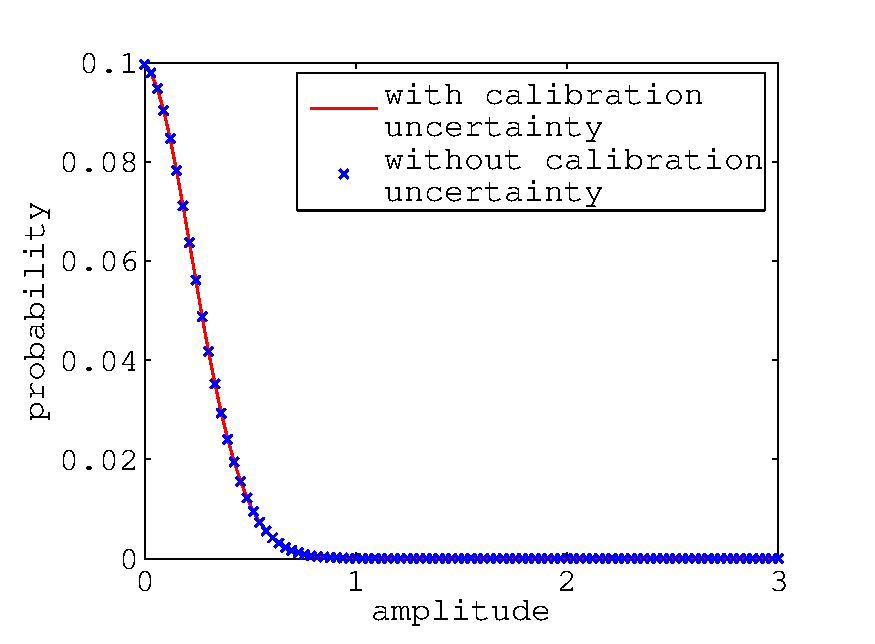
\includegraphics[width=0.6\textwidth]{figs/MargCalibUncert}\caption[Marginalised
calibration uncertainty.]{Comparison of pdfs calculated with a calibration uncertainty as in
equation~\ref{MargCalibUncertEqn} compared to that from equation~\ref{StudentstLikelihood} without
the calibration uncertainty.}\label{MargCalibUncert}
\end{center}
\end{figure}
The use of a Jeffreys prior for $\lambda$ would make little difference, with it just making the
factor in equation~\ref{MargCalibUncertEqn} $1/\lambda^{2m_j-1}$. This result is not too
surprising as if the value is just random noise with equal probability over an equal range either
side of the obtained value then that value will stay the most probable.

\subsubsection{Distance errors}
Another area of uncertainty is the distance to the pulsar. This is required when calculating the
pulsars ellipticity. There are a variety of ways to measure pulsar distances, with the two main
distance indicators being parallax, for nearby objects, and interstellar dispersion, for more
distant sources. Measurements made using the dispersion measure make use of a model of the
distribution of electron density within the galaxy, with the current best model being that of Taylor
and Cordes (1993) \cite{TaylorCordes:1993}. Despite this there are still errors of about 10\% on
most measurements (see review of pulsar distance measurements in Frail and Weisberg, 1990
\cite{Frail:1990}). The majority of pulsar distance measurements provided in \cite{ATNF} make use of
the Taylor and Cordes model, but it otherwise gives the best estimate. Plots of the pulsar distances
from the Earth are shown in figure~\ref{PulsarDist}.
\begin{figure}[!htbp]
\caption[Best estimate distances in kpc from the Earth for 92 pulsars.]{Best estimate distances
in kpc from the Earth for our 92 pulsars \cite{ATNF} (PSR\,J0537-6910 is left out as it is very
distant in the LMC), where $x=r\cos{\delta}\cos{\alpha}$, $y = r\cos{\delta}\sin{\alpha}$ and $z =
r\sin{\delta}$ are the normal conversions between spherical polar and Cartesian coordinates. The
magenta circles represent pulsars in globular clusters.}\label{PulsarDist}
\begin{center}
\begin{tabular}{c}
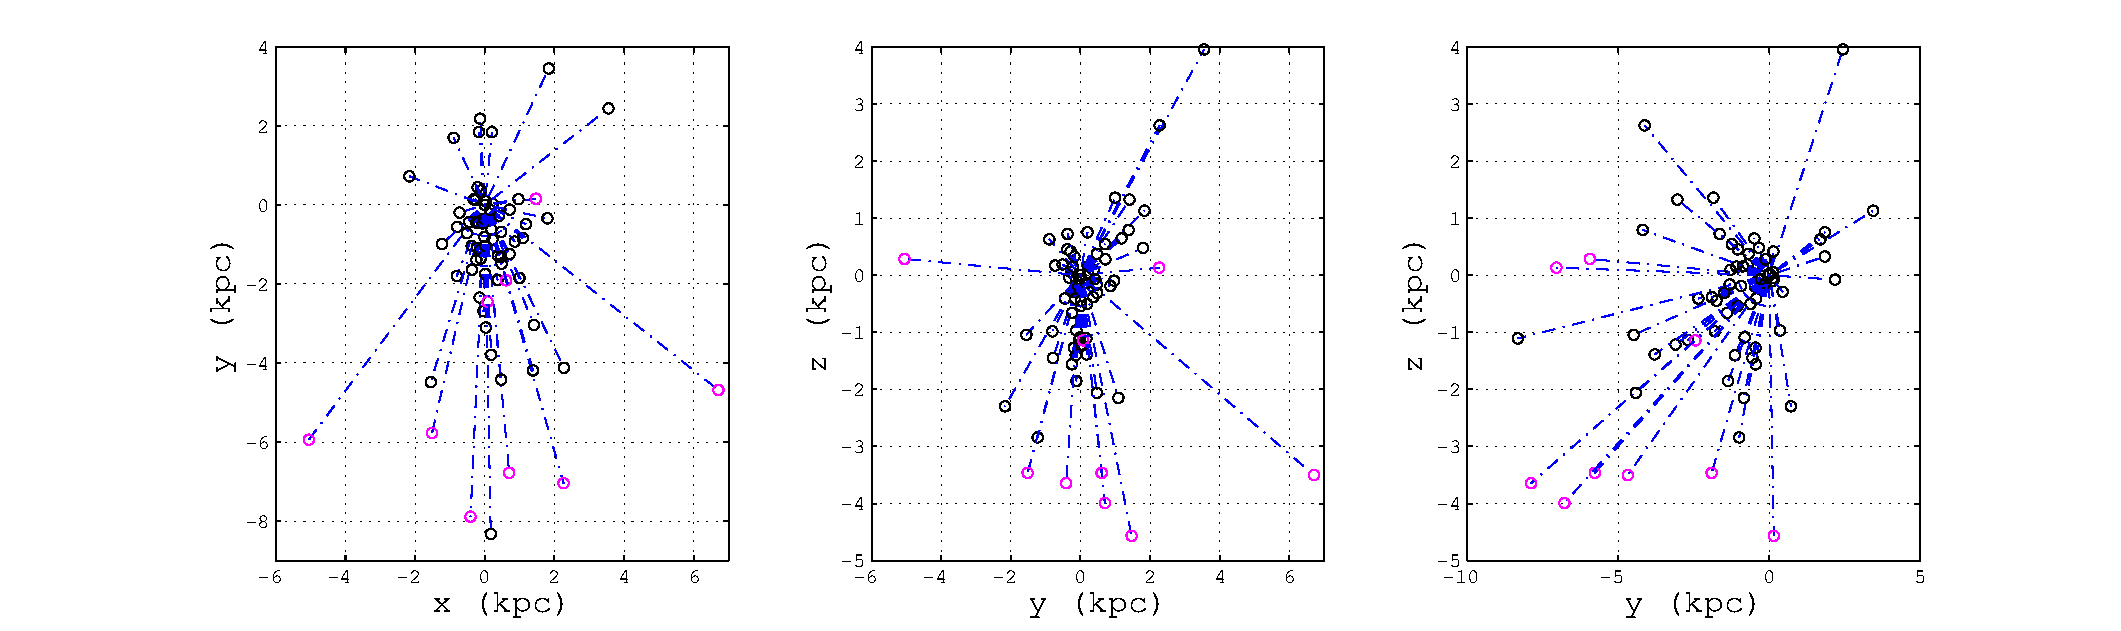
\includegraphics[width=1.0\textwidth]{figs/PulsarDistCart} \\
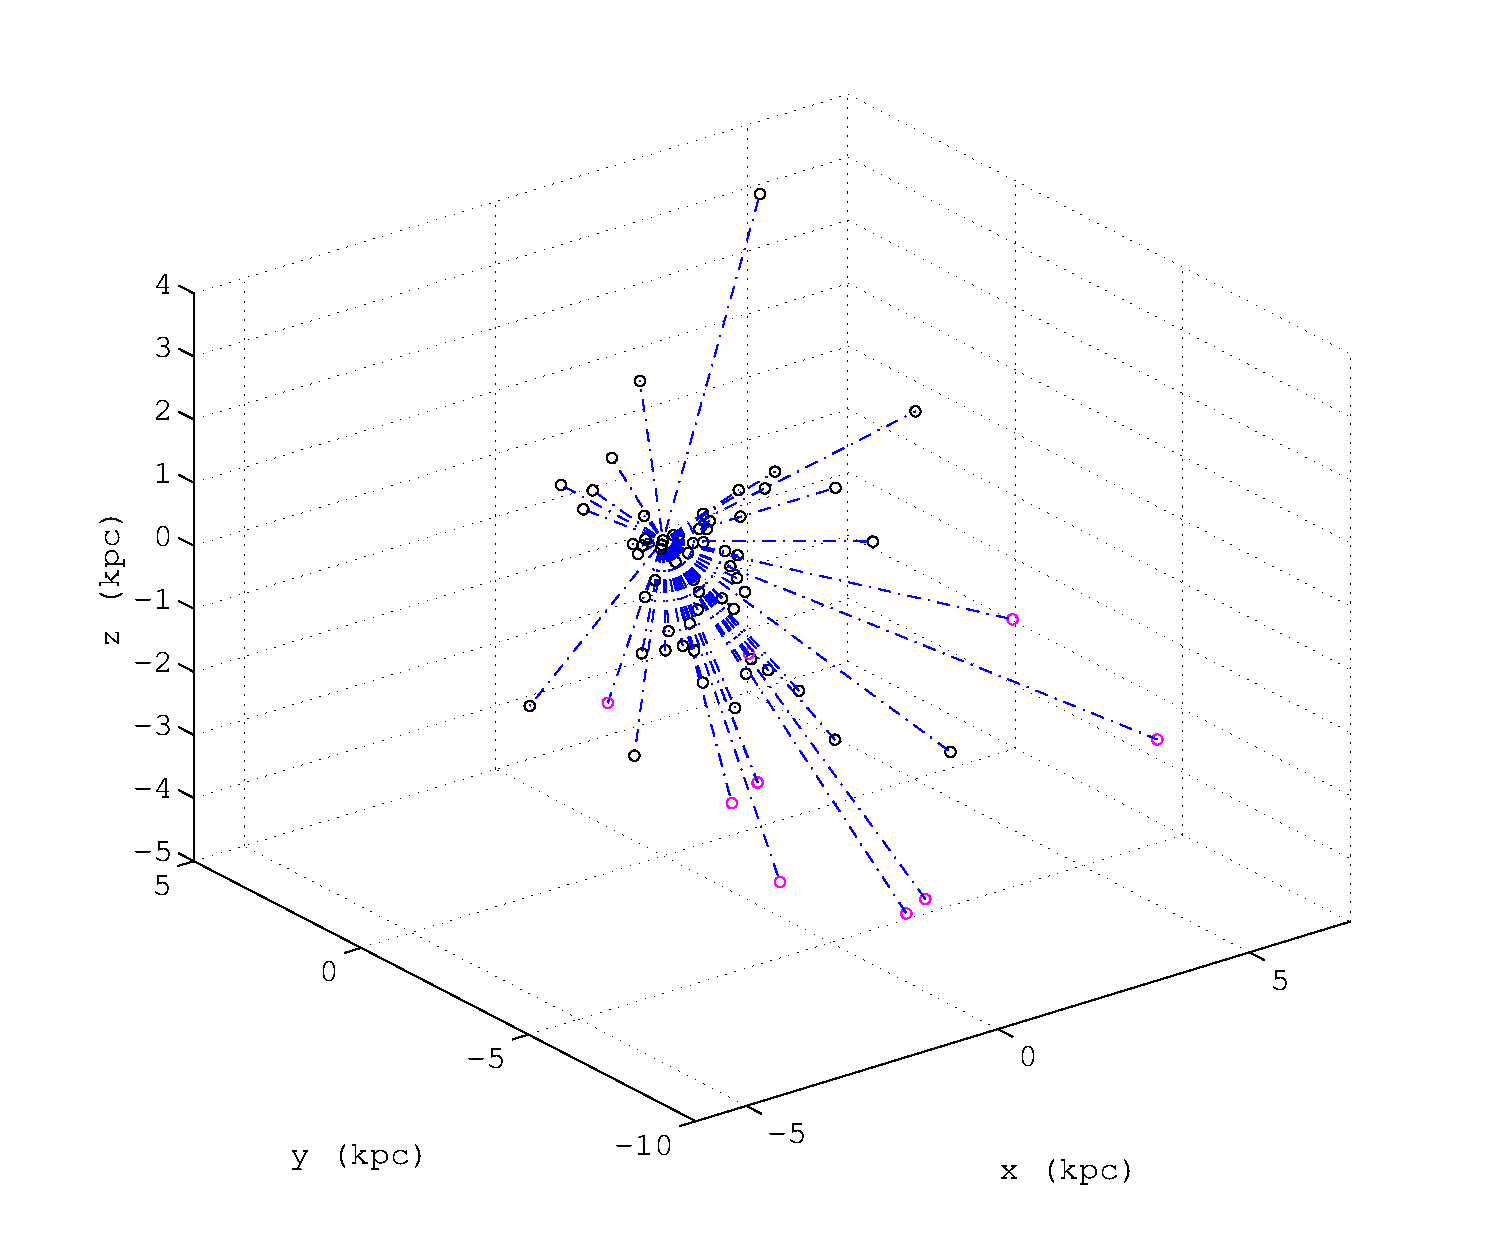
\includegraphics[width=0.6\textwidth]{figs/PulsarDist3D}
\end{tabular}
\end{center}
\end{figure}

As with the calibration uncertainty we can take a similar view of the distance uncertainty,
although this also requires a change of variable. We will assume that the distance error is a
random number within a given distribution symmetric about the best estimate. To change variables
from $h_0$ to $\varepsilon$ the pdf is
\begin{equation}
p(\varepsilon|r) = p(h_0|r)\frac{{\rm d}h_0}{{\rm d}\varepsilon},
\end{equation}
which from differentiating equation~\ref{h0epsilon} gives
\begin{equation}
p(\varepsilon|r) \propto \frac{p(h_0|r)}{r}.
\end{equation}
From this we get
\begin{eqnarray}
p(\varepsilon,r) & = & p(\varepsilon|r)p(r), \nonumber \\
& \propto & \frac{p(h_0|r)}{r}p(r), \nonumber \\
p(\varepsilon) & \propto & \int \frac{p(h_0|r)}{r}p(r) {\rm d}r,
\end{eqnarray}
which given a uniform distribution for $p(r)$ over a range $r_{\rm min}$ to $r_{\rm max}$,
where $r_{\rm min} = r - 0.1r$ and $r_{\rm max} = r + 0.1r$ (assuming 10\% errors from the best
fit distance $r$), just gives $p(\varepsilon) \propto p(h_0)$. This is intuitively the case as if
there is an equal probability that the pulsar is slightly closer or slightly further away, then the
most probabilistically likely value would be the best fit value. This would be the same if  the
prior $p(r)$ were a Gaussian distribution about the best fit value. If there were not equal
probability either side of the best fit this would not be the case, but for all our distance errors
we shall assume it is.

\subsection{S3}
The S3 run was partaken with the three LIGO interferometers and G\textsc{eo}\,600. These detectors
had different duty cycles and sensitivities over the run. The collocated H1 and H2 interferometers
maintained a relatively high duty cycle of $\sim 69.3\%$ and $\sim 63.4\%$
respectively\footnote{\url{http://www.phys.lsu.edu/faculty/gonzalez/S3LockStats/}}. The L1
interferometer was badly affected by anthropogenic noise sources during the day and thus had a
relatively poor duty cycle of $\sim 21.8\%$. The \geo interferometer did not operate for the full
time of S3, but had two main data taking periods between which improvements were made to its
sensitivity. These were from $5^{\rm th}$ to $12^{\rm th}$ November 2003, called S3\,I, and $30^{\rm
th}$ December 2003 to $13^{\rm th}$ January 2004, called S3\,II. Typical sensitivities for these can
be seen in figure~\ref{S3SensitivityCurves}.
\begin{figure}[!htbp]
\begin{center}
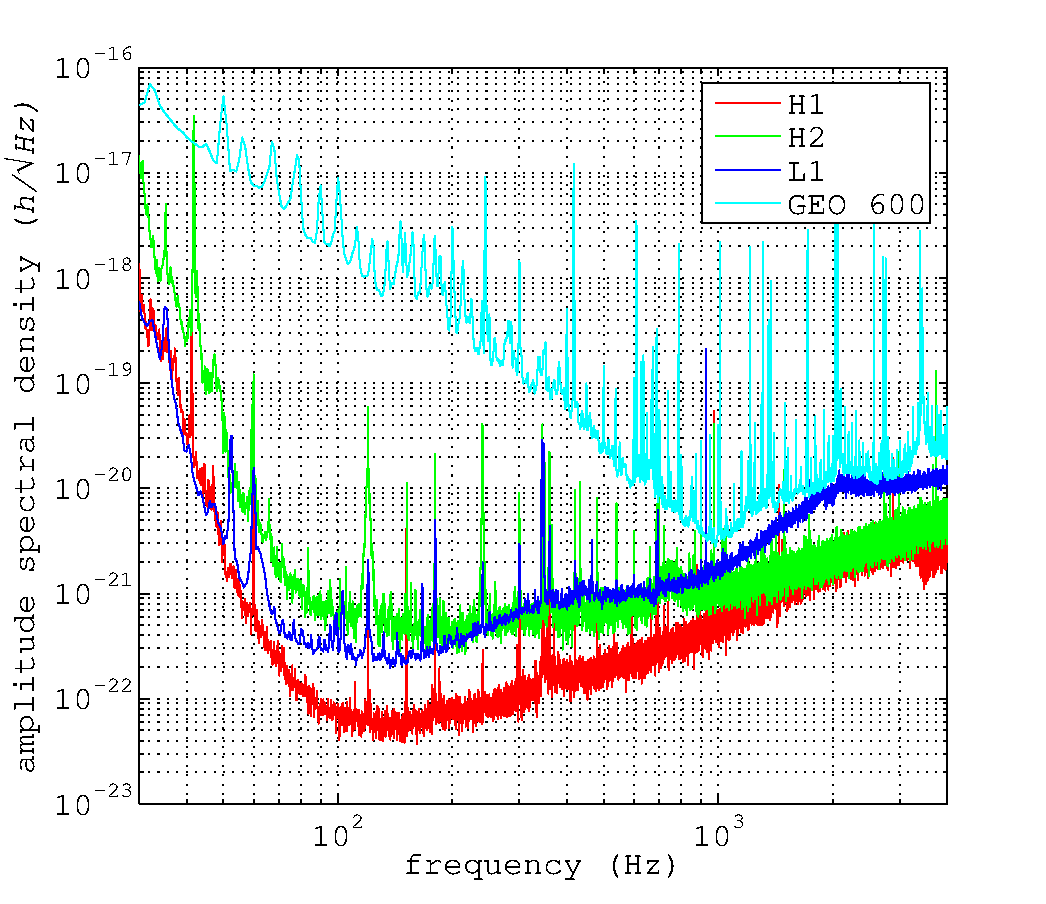
\includegraphics[width=0.6\textwidth]{figs/S3SensitivityCurves}\caption[Typical sensitivity curves
for the LIGO and \geo interferometers over the period of S3.]{Typical sensitivity curves for the
LIGO and \geo interferometers over the period of S3. These curves have been reproduced using the
official LIGO and \geo sensitivities from \cite{LIGOsensitivity,
GEOsensitivity}.}\label{S3SensitivityCurves}
\end{center}
\end{figure}
It can be seen that \geo only competes with the LIGO detectors for frequencies $\gtrsim 1$\,kHz,
where the signal recycling was tuned to. The LIGO detectors have their best sensitivities between
$\sim 100$ and 200\,Hz.

The S3 injections suggest that there is phase consistency between the LIGO detectors, which allows a
joint analysis combining the data from all interferometers. For all but one pulsar (PSR\,J1939+2134,
the, until recently, fastest millisecond pulsar with $\nu_{\rm gw} \sim 1283.9$\,Hz) it was not
worth including \geo data in the joint analysis. The phase coherence of \geo with the LIGO
interferometers was checked in \cite{Dupuis:2004}. The results of $h_0^{95\%}$ for each LIGO
interferometer and the joint results, including ellipticity (assuming $I_{zz} = 10^{38}\,{\rm
kg}\,{\rm m}^2$ and the best estimate distances from \cite{ATNF}) are given in
table~\ref{S3Results}. The results for PSR~J1939+2134 including \geo in the joint analysis are given
in table~\ref{S3ResultsPlusGEO}.
\input bigtables/S3ResultsTable.tex
\begin{table}[!htbp]
\caption{\label{S3ResultsPlusGEO} The S3 results for PSR\,J1939+2134 including \geo.}
\begin{center}
\begin{tabular}{ l | c  | c |  c | l }
\footnotesize{P\textsc{ulsar}} &  \footnotesize{$h_0^{95\%}$ \geo} & \footnotesize{$h_0^{95\%}$
Joint} & \footnotesize{$\varepsilon$} & \footnotesize{spin-down UL ratio} \\ 
\hline \hline 
\scriptsize{\tt{J1939+2134}} & \scriptsize{$\tt{8.5\ee{-23}}$} & \scriptsize{$\tt{5.0\ee{-24}}$} &
\scriptsize{$\tt{1.0\ee{-5}}$} & \scriptsize{$\tt{2732^{\dagger}}$} \\[-16pt]
\end{tabular}
\end{center}
\end{table}
It can be seen in table~\ref{S3ResultsPlusGEO} that including \geo in the analysis does not add
significantly to the results.

\subsection{S4}
Between S3 and S4 the L1 interferometer was upgraded with better seismic isolation. This greatly
reduced the amount of time the interferometer was thrown out-of-lock by anthropogenic noise, and
allowed it to operate successfully during the day, with a duty cycle of $\sim 74.5\%$ and a longest
lock stretch of 18.7\,hours. The H1 and H2 interferometers also both improved their duty cycles to
$\sim 80.5\%$ and $\sim 81.4\%$, with longest lock stretches of almost a day. The best
sensitivities for all the detectors during S4 can be seen in figure~\ref{LIGO_GEO_S4_STRAIN}.
\begin{figure}[!htbp]
\begin{center}
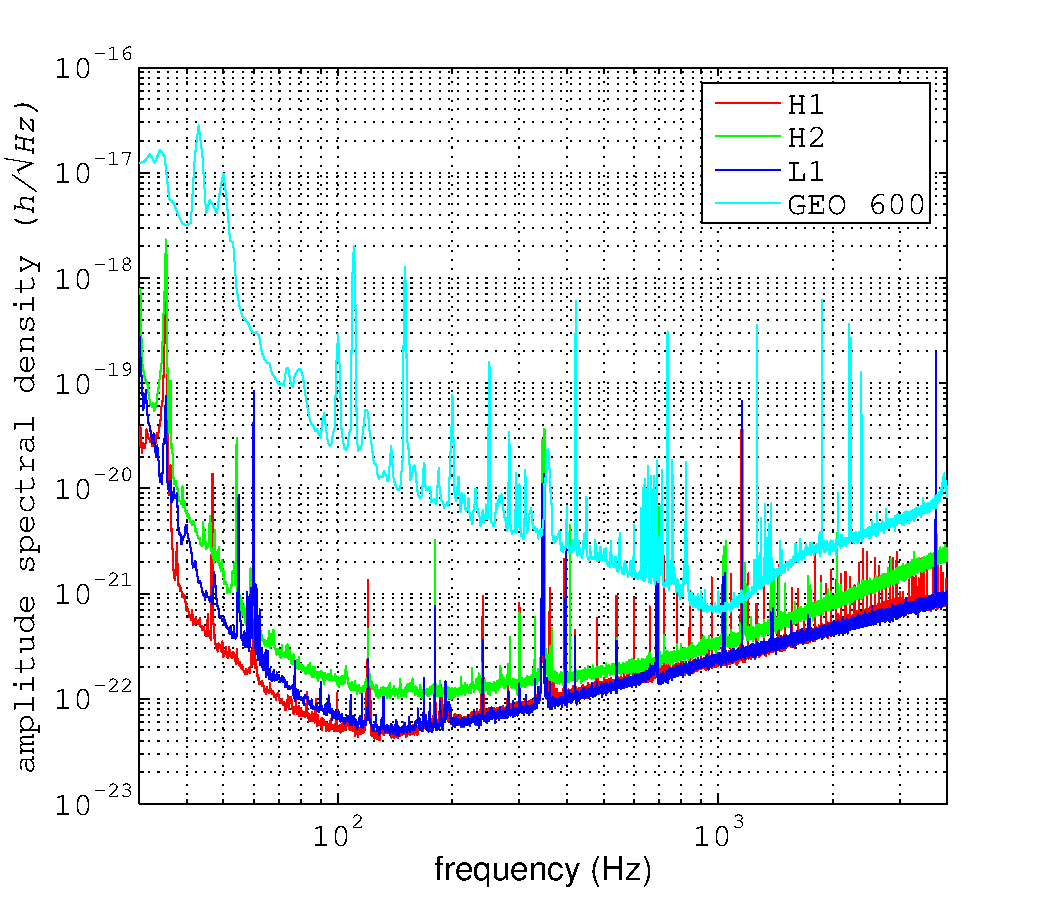
\includegraphics[width=0.6\textwidth]{figs/LIGO_GEO_S4_STRAIN}\caption[Best sensitivities of the
LIGO and \geo detectors during S4.]{Best sensitivities of the LIGO and \geo detectors during S4.
These curves have been reproduced using the official LIGO and \geo sensitivities from 
\cite{LIGOsensitivity, GEOsensitivity}.}\label{LIGO_GEO_S4_STRAIN}
\end{center}
\end{figure}

The results of the S4 analysis for the LIGO interferometers is given in table~\ref{S4Results}.
%Due to the calibration phase error of $\pi$\,rads in H1 and H2 (see \S\ref{S4injections}) these
%have been produced using $B_k$s corrected for this by multiplying them by $-1$. When the final
%calibrations becomes available the results will be reproduced with those. 
For S4 the \geo interferometer provided two pulsars on a comparable scale to LIGO: PSR\,J1939+2134
and PSR\,J1843-1113. At present there has been no test of the phase consistency of the LIGO and \geo
interferometers during S4, although there is no reason to believe they are not coherent - no
hardware injection was made in \geo for S4.
\input bigtables/S4ResultsTable.tex
The results with the two pulsars for which \geo has been included are given in
table~\ref{S4ResultsPlusGEO}.
\begin{table}[!htbp]
\caption{\label{S4ResultsPlusGEO} The S4 results including \geo.}
\begin{center}
\begin{tabular}{ l | c  | c |  c | l }
\footnotesize{P\textsc{ulsar}} &  \footnotesize{$h_0^{95\%}$ \geo} & \footnotesize{$h_0^{95\%}$
Joint} & \footnotesize{$\varepsilon$} & \footnotesize{spin-down UL ratio} \\ 
\hline \hline
\scriptsize{\tt{J1843-1113}} & \scriptsize{$\tt{3.8\ee{-23}}$} & \scriptsize{$\tt{1.8\ee{-24}}$} &
\scriptsize{$\tt{2.8\ee{-6}}$} & \scriptsize{\tt{1875}} \\[-7pt]
\scriptsize{\tt{J1939+2134}} & \scriptsize{$\tt{2.6\ee{-23}}$} & \scriptsize{$\tt{2.4\ee{-24}}$} &
\scriptsize{$\tt{4.9\ee{-6}}$} & \scriptsize{$\tt{1300^{\dagger}}$} \\
\end{tabular}
\end{center}
\end{table}
It can be seen that \geo adds only fractionally to the overall sensitivity for PSR\,J1843-1113.

\subsection{S3 and S4}
Our analysis technique allows us to combine the data from different runs in a way similar to the
ability to combine data from all the interferometers to create a joint results. This becomes
useful when runs are of a similar sensitivity, which is the case for areas of the frequency
spectrum for S3 and S4. The data can be combined by simply concatenating the separate calibrated
$B_k$ files together. This is valid provided that the calibration phase is consistent between runs.

The results for the LIGO interferometers are given in table~\ref{S3S4Results}.
\input bigtables/S3S4ResultsTable.tex
\geo was included in the joint analysis for the same two pulsars as the S4 results (see
table~\ref{S3S4ResultsPlusGEO}).
\begin{table}[!htbp]
\caption{\label{S3S4ResultsPlusGEO} The combined S3 and S4 results including \geo.}
\begin{center}
\begin{tabular}{ l | c  | c |  c | l }
\footnotesize{P\textsc{ulsar}} &  \footnotesize{$h_0^{95\%}$ \geo} & \footnotesize{$h_0^{95\%}$
Joint} & \footnotesize{$\varepsilon$} & \footnotesize{spin-down UL ratio} \\ 
\hline \hline
\scriptsize{\tt{J1843-1113}} & \scriptsize{$\tt{3.7\ee{-23}}$} & \scriptsize{$\tt{1.6\ee{-24}}$} &
\scriptsize{$\tt{2.5\ee{-6}}$} & \scriptsize{\tt{1671}} \\[-7pt]
\scriptsize{\tt{J1939+2134}} & \scriptsize{$\tt{2.5\ee{-23}}$} & \scriptsize{$\tt{2.0\ee{-24}}$} &
\scriptsize{$\tt{4.1\ee{-6}}$} & \scriptsize{$\tt{1071^{\dagger}}$} \\
\end{tabular}
\end{center}
\end{table}
For the vast majority of pulsars combining the two runs improves the results, although for a few
the S3 data has a detrimental effect (of a few percent) with the S4 data providing the lowest upper
limit.

The upper limits on $h_0$ and $\varepsilon$ from the S3, S4 and the combined data set are plotted in
figures~\ref{h0results}
and \ref{ellresults}.
\begin{figure}[!htbp]
\begin{center}
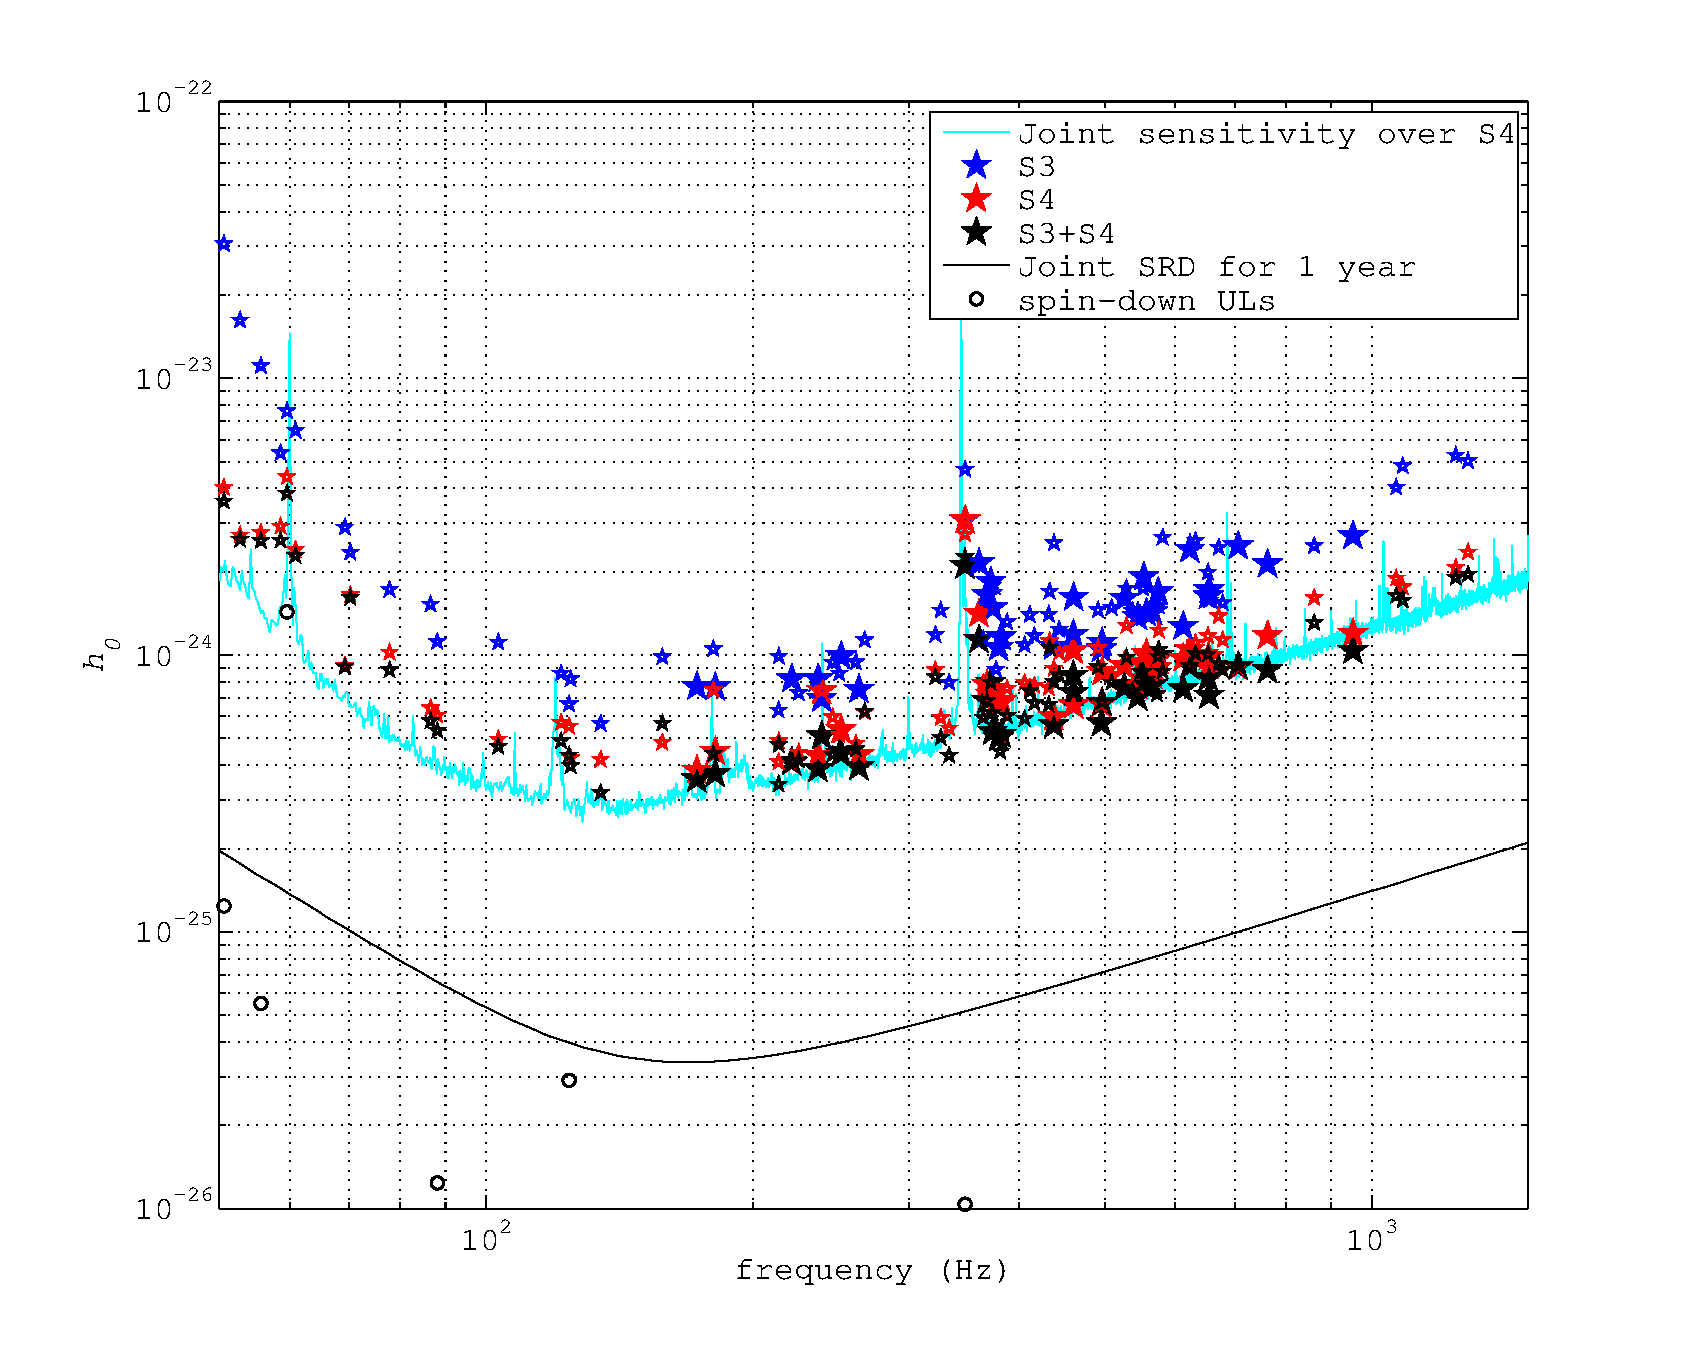
\includegraphics[width=1.0\textwidth]{figs/upperlimits}\caption[95\% upper limits on $h_0$ for 93
pulsars using the S3, S4 and combined data sets.]{95\% upper limits on $h_0$ for 93 pulsars using
the S3, S4 and combined data sets. Bold stars represent pulsars within globular clusters. Also shown
is the joint LIGO upper limit estimated from their best noise spectral densities during S4. A joint
upper limit estimate for LIGO using their design (SRD) sensitivities integrated over one year is
shown. Several pulsar spin-down upper limits are also shown for those within the range of the
figure.}\label{h0results}
\end{center}
\end{figure}
\begin{figure}[!htbp]
\begin{center}
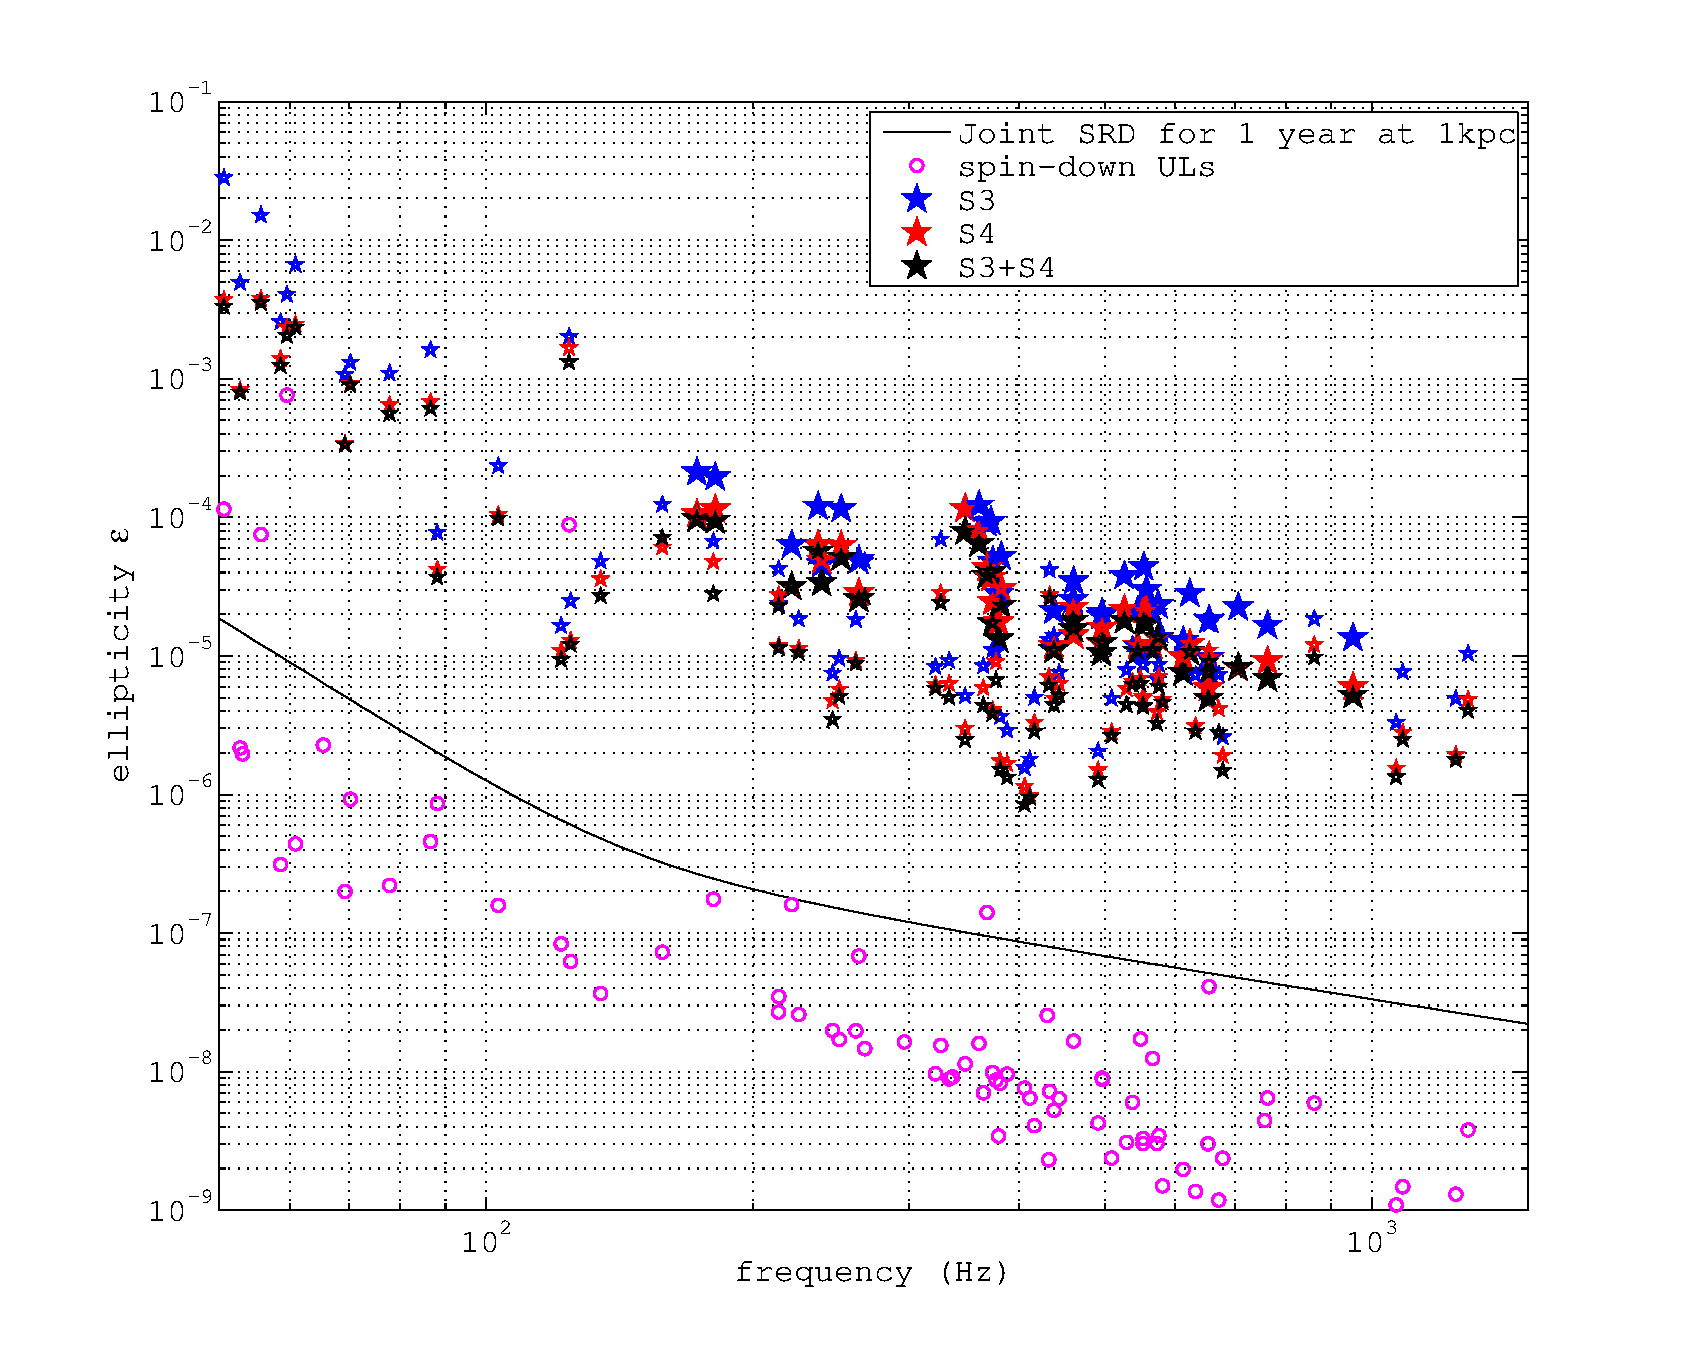
\includegraphics[width=1.0\textwidth]{figs/upperlimitsEll}\caption[Upper limits on pulsar
ellipticity for the S3, S4 and combined data sets.]{Upper limits on pulsar ellipticity for the S3,
S4 and combined data sets. Bold stars represent pulsars within globular clusters. Also shown is the
ellipticity limit that could be produced using the joint design sensitivity upper limit integrated
over one year for a source at a distance of 1\,kpc. The spin-down upper limits are also
plotted.}\label{ellresults}
\end{center}
\end{figure}
Figure~\ref{h0results} also shows an estimate of the upper limit across the frequency range by
combining the LIGO noise spectral density sensitivity curves, taken as the best sensitivity during
S4. The estimate is made using the relation $h_0^{95\%} = 10.8\sqrt{S_h(f)/T_{\rm obs}}$, where
$S_h(f)$ is the one-sided power spectral density (PSD) and $T_{\rm obs}$ is each detector's live
time (using the associated duty cycle of each interferometer during the run). The factor 10.8, given
in Dupuis and Woan (2005) \cite{DupuisWoan:2005}, has been modified from the value of 15.3
calculated in \cite{Dupuis:2004} from simulations using white noise averaged over sky position, due
to an error in the definition of the noise spectral density. The joint upper limit curve is produced
by combining the detector PSDs via
\begin{eqnarray}
S(f) & = & \left(\frac{T_{\rm obs~H1}}{S_h(f)_{\rm H1}} + \frac{T_{\rm obs~H2}}{S_h(f)_{\rm
H2}} + \frac{T_{\rm obs~L1}}{S_h(f)_{\rm L1}} \right)^{-1} \\ \nonumber
h_0^{95\%} & = & 10.8\sqrt{S(f)}.
\end{eqnarray} 
In \cite{Abbott:2005} a similar plot to figure~\ref{h0results} is shown for the S2 data using a
factor of 11.4 in the relation between the upper limit and PSD. This definition comes from using the
$\mathcal{F}$-statistic search method and setting a 1\% false alarm rate and 10\% false dismissal
rate for signals given the underlying detector PSD. It can be seen that the majority of the combined
S3 and S4 upper limits are dominated by the S4 data, with a few for which the S4 data alone
produces the more stringent upper limit. Combining the data set has pushed two of the ellipticity
limits below the level of $10^{-6}$. The implications of these results will be discussed in
\S\ref{astrophysics}.

\subsection{Moment of inertia - ellipticity plane}
The moment of inertia of a neutron star will depend on the equation-of-state (EOS) used to model it.
For all the above results on pulsar ellipticity a moment of inertia of $10^{38}\,{\rm kg}\,{\rm
m}^2$ has been assumed (see Chapter~2), which relies upon a particular equation-of-state being
correct. It also assumes a neutron star mass of $1.4\,M_{\odot}$. For many known radio pulsars in
binary systems, where the mass can be measured, this mass estimate appears to be remarkably well
kept (see Thorsett and Chakrabarty, 1999 \cite{Thorsett:1999}). Recent measurements have reported
two of the most massive pulsars known with Nice {\it et al.} (2005) \cite{Nice:2005} giving the
highest recorded pulsar mass at $2.1\,M_{\odot}$, although with wide error bars, and Ransom {\it et
al.} (2005) \cite{Ransom:2005} giving a mass of $1.68\,M_{\odot}$ at 95\% confidence.
There are many equations-of-state, some considered more realistic (using nucleons and leptons) and
others considered less likely (involving more exotic particles or quark states), giving moments of
inertia varying over factors of about two, with Thorne (1987) \cite{300Years} giving a range for
different EOS of $3\ee{37}$\,kg\,${\rm m}^2 \lesssim I_{zz} \lesssim 3\ee{38}$\,kg\,${\rm m}^2$. The
high mass neutron stars given above could possible have ellipticities towards the high end of this
range. Attempts have been made by Bejger and Haensel (2002 and 2003) \cite{Bejger:2002, Bejger:2003}
to set limits on the moment of inertia of the Crab pulsar by equating its spin-down energy loss to
the expansion of the Crab nebula and its electromagnetic emission, which have been used to confine
its mass and radius. More recently Bejger {\it et al.} (2005) \cite{Bejger:2005} have set
constraints on the moment of inertia of the neutron stars in the double pulsar binary system
PSRs\,J0737-3039A and B giving values close to the canonical value.

As suggested in Pitkin {\it et al} (2005) \cite{Pitkin:2005} instead of using
equation~\ref{h0epsilon} to set a limit on $\varepsilon$ directly it can be used to set a limit on
the neutron star quadrupole moment $I\varepsilon$, which does not contain the mass and moment of
inertia assumptions. The quadrupole moment can then be used to provide constraints on an
$I-\varepsilon$ plane with exclusion regions. With this plane, an upper limit on $\varepsilon$ can
then be read off using your favoured equation-of-state. The spin-down upper limit can also be used
to provide exclusion regions via the relation
\begin{equation}
I_{zz} = \frac{5|\dot{\Omega}|c^5}{32G\Omega^5}\frac{1}{\varepsilon^2}.
\end{equation}

For most pulsars, forming an $I-\varepsilon$ plane will generally provide very little more
information than the straight limit set with the canonical moment of inertia when compared to the
spin-down limit. For the Crab pulsar and PSR\,J0537-6910, which are nearing their spin-down
limits, it starts to become more interesting with the experimental values nearing the point where
they beat the spin-down limit for moments of inertia from exotic equations-of-state\footnote{This
is not to say that they are compatible with ellipticities obtainable with exotic EOSs which are
generally a few orders of magnitude smaller.}. In the following sections the results for these two
pulsars are discussed.

There are a couple of other constraints which can be placed on the $I-\varepsilon$ plane (see
figure~\ref{Ieplane}). The first constraint is that from the EOS. These provide limits on the
possible mass and radius of neutron stars and can provide upper and lower limits on the range of
moments of inertia. They will also constrain the maximum ellipticity that the neutron star could
sustain, estimates of which for various neutron star equations of state are given by Owen (2005)
\cite{Owen:2005}. For the Crab pulsar a lower limit can be placed on the moment of inertia by
equating its loss in rotational energy with the energetics of the Crab nebula surrounding it
(discussed below) \cite{Bejger:2003}.
\begin{figure}[!htbp]
\begin{center}
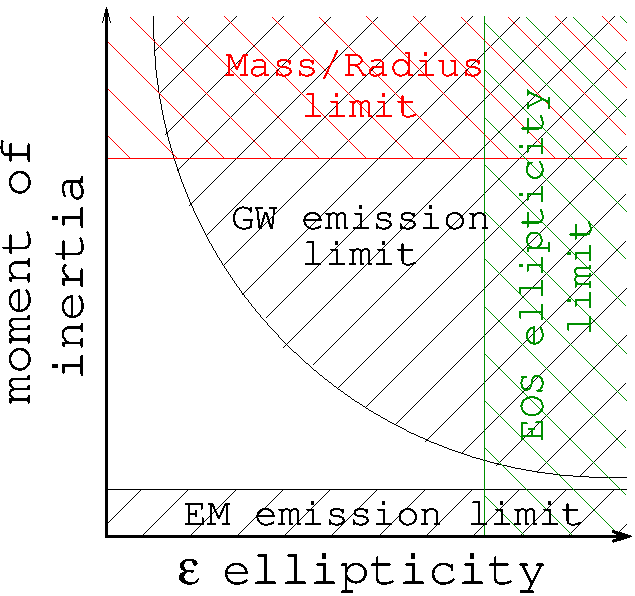
\includegraphics[width=0.55\textwidth]{figs/Ieplane}\caption[The regions in the moment of inertia
$I_{zz}$-$\varepsilon$ plane for a pulsar that can be excluded via various methods.]{The regions in
the moment of inertia $I_{zz}$-$\varepsilon$ plane for a pulsar that can be excluded via various
methods. The electromagnetic emission of a pulsar can set a lower limit on the moment of inertia by
equating the EM emission with the rotational energy loss of the pulsar. The various
equations-of-state for neutron stars can constrain the mass/radius relation and therefore moment of
inertia \cite{Lattimer:2001}. Equations of state will also put limits on the maximum allowable
ellipticity of the neutron star. A limit can be set from upper limits on gravitational wave
emission.}\label{Ieplane}
\end{center}
\end{figure}

\subsection{The Crab pulsar}\label{CrabPulsarResults}
Of the known radio pulsars, the Crab pulsar has often been considered one of the most promising
sources of gravitational waves. This is in part due to its youth and therefore large spin-down rate,
leading to a relatively large spin-down upper limits orders of magnitude higher than for most other
pulsars. The high rate of glitching in the pulsar also provides possible evidence of asymmetry. One
glitch model, favoured for the Crab pulsar, is that there is a change in the pulsar ellipticity, and
breaking of the crust, as the star settles to its new equilibrium state as it spins-down
\cite{PulsarAstronomy}. Back in the 1970s estimates of \gw strains were spurred on by the
experimenters producing novel technologies which could start the possibility of probing these low
strains, with Zimmermann (1978) \cite{Zimmermann:1978} producing estimates of \gw strains from the
Crab pulsar ranging from $2\ee{-25} \lesssim h_0 \lesssim 2\ee{-29}$. 

The first searches for \gws from the Crab pulsar were by the Japanese using specially designed
resonant bar detectors, with frequencies of around 60\,Hz \cite{Hirakawa:1978}. The most recent
result using such a bar was from 1993 and gave a $1\sigma$ upper limit of $h_0 \le 2\ee{-22}$
\cite{Suzuki:1995}. This upper limit has now been overtaken with the advent of the
interferometric \gw detectors, with results of the S2 run, giving $h_0^{95\%} = 4.1\ee{-23}$
\cite{Abbott:2005}. Using equation~\ref{spindownUL}, and taking $I_{zz}=10^{38}$\,kg\,${\rm m}^2$
and $r = 2$\,kpc, gives a spin-down upper limit for the Crab pulsar of $h_0 < 1.4\ee{-24}$. This
meant that for S2 the Crab pulsar results was still a factor of $\sim 30$ above the spin-down limit.
This was still the closest result to the spin-down upper limit so far obtained and closest of any of
the known pulsars searched for.

The Crab pulsar does require special attention. As described in Chapter 2 the effect of timing
noise has to be taken into account. Also its \gw frequency sits very close to 60\,Hz, which is the
mains AC frequency in the US, so checks need to be made that this line, as appearing in the detector
spectra, does not interfere with the analysis. Figure~\ref{CrabSpectrum} shows the spectra around
the 60\,Hz for the LIGO interferometers during a section of S3 and S4. It can be seen that the
60\,Hz power line does not seem to interfere with the data at the Crab pulsar frequency of $\sim
59.6$\,Hz.
\begin{figure}[!htbp]
\begin{tabular}{l l}
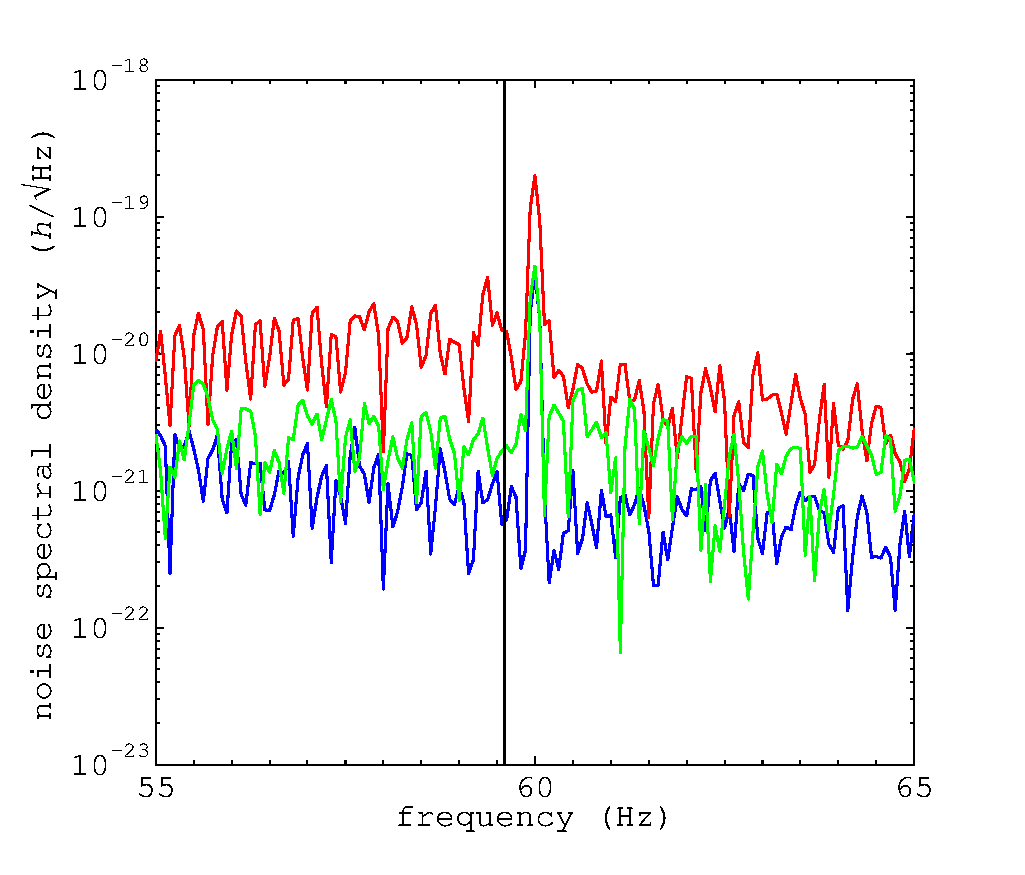
\includegraphics[width=0.45\textwidth]{figs/S3CrabSpectrum} &
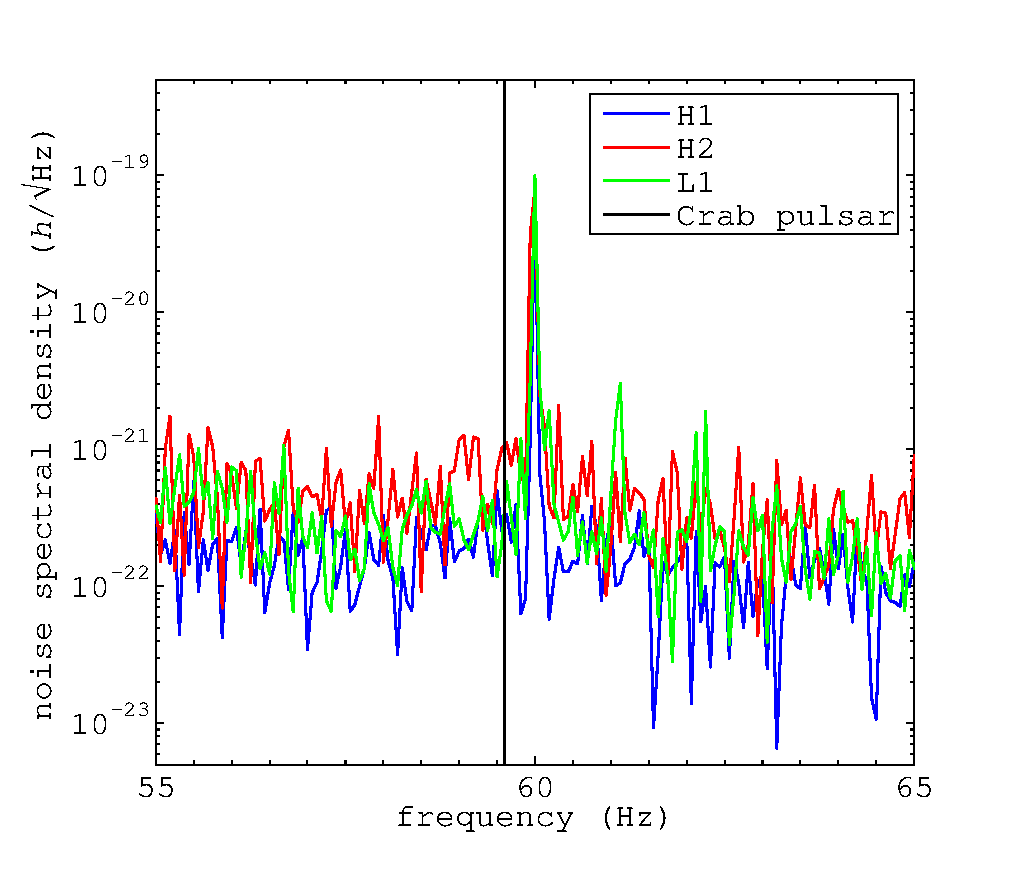
\includegraphics[width=0.45\textwidth]{figs/S4CrabSpectrum}
\end{tabular}\caption[The LIGO noise spectral densities between 55 and 65\,Hz for S3 and S4.]{The
LIGO noise spectral densities between 55 and 65\,Hz for S3 (left) and S4 (right) showing the 60\,Hz
power line and Crab pulsar frequency.}\label{CrabSpectrum}
\end{figure}

The general results for the Crab pulsar can be seen with the others in tables~\ref{S3Results},
\ref{S4Results} and \ref{S3S4Results}. It can be seen that the results improve by about an order of
magnitude over those from the previous S2 run. The majority of this improvement was between the S2
and S3 runs, with there not being as big an improvement in the low frequencies between S3 and S4.
The results for the Crab pulsar over the S2, S3 and S4 runs are plotted on the $I-\varepsilon$ plane
in figure~\ref{CrabIeplane}.
\begin{figure}[!htbp]
\begin{center}
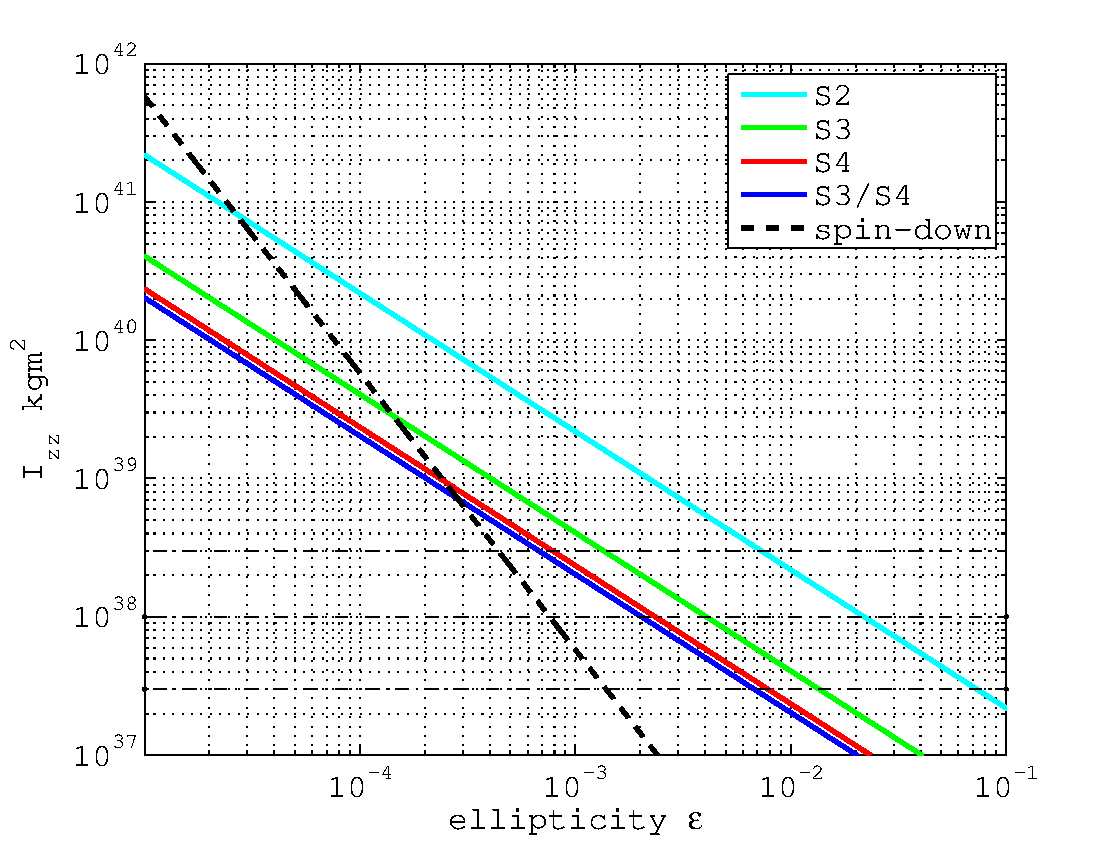
\includegraphics[width=0.6\textwidth]{figs/CrabIeplane}\caption{The moment of inertia-ellipticity
plane for the Crab pulsar over the S2, S3 and S4 runs.}\label{CrabIeplane}
\end{center}
\end{figure}
It can be seen that over the range of $3\ee{37} < I_{zz} < 3\ee{38}\,{\rm kg}\,{\rm m}^2$, which
covers moments of inertia from even some of the most exotic EOS, that the ratio of the spin-down
upper limit to our results ranges from $\sim 5$ at the lower end to $\sim 1.5$ at the upper end. For
the Crab pulsar the spin-down limit argument is rather spurious as it is known that at least some of
the spin-down energy goes into the energetics of the Crab nebula. The fact that the braking index
of the pulsar is not 3, but 2.51, shows that it is not spinning down purely through magnetic dipole
radiation. In Palomba (2000) \cite{Palomba:2000} several reasons for having $n \ne 3$ are mentioned,
including particle acceleration in pulsar winds or non-dipole magnetic fields, but in particular
there is discussion of the effects of gravitational radiation. If the spin-down were purely through
emission of \gws one would expect $n=5$, so Palomba (2000) \cite{Palomba:2000} tries combining all
possible mechanisms of producing $n=2.51$ to provide limits on the \gw emission. This gives an upper
limit of $\varepsilon \le 3\ee{-4}$, which is 2.5 times lower than the previous spin down limit
(assuming all emission via gravitational waves) and therefore makes our result over six times
greater than this new upper limit.

For these results we have assumed that the $\alpha$ parameter of Jones (2004) \cite{Jones:2004} has
a value of 1, i.e. the \gw and electromagnetic timing noise of the Crab pulsar are the same. As
previously stated this seems to be a good assumption, although when our results start to beat the
spin-down limit it could be worth including this as an extra parameter in the search.

\subsection{PSR\,J0537-6910}\label{PSRJ0537-6910section}
Another interesting pulsar worth closer study is PSR\,J0537-6910. This pulsar, associated with the 
SNR N157B in the Large Magellanic Cloud (LMC), is currently only seen as an X-ray pulsar and is
the fastest rotating young pulsar, with a rotation frequency of $\sim 62$\,Hz \cite{Marshall:2004}.
It is also one of the most prolific glitchers of the known pulsars, with a rate of 2.3 per year seen
over the period of study in Marshall {\it et al.} (2004) \cite{Marshall:2004} (with a number of
observations using the {\it Rossi X-ray Timing Explorer} between $19^{\rm th}$ January 1999 and
$23^{\rm rd}$ August 2001). Despite this high glitch rate Marshall {\it et al.} (2004)
\cite{Marshall:2004} were able to carry out phase-connected timing solutions between glitches and
get measurements of ${\ddot{\nu}}$ and therefore the braking index $n$. The observed value of
$n \ge 6.9$ is well away from the pure dipole radiation value of 3, although as stated in
\cite{Marshall:2004} there could be some contamination due to timing noise and uncertainties in the
pulsars position and the $\ddot{\nu}$ value. We have not been able to obtain timing data for this
pulsar over the periods of S3 and S4, so the high glitch rate and unknown timing noise mean these
results should be accepted as possibly invalid. It also has potential problems with the frequency
parameter errors pushing its maximum phase error over our $30^{\circ}$ limit. Its parameters taken
from \cite{Marshall:2004}, and as used for the heterodyne procedure (at twice the frequency), are
given in table~\ref{J0537-6910Params}.
\begin{table}[!htbp]
\caption{\label{J0537-6910Params} The parameter values for PSR\,J0537-6910.}
\begin{center}
\begin{tabular}{| c | l |}
\hline
\multicolumn{2}{| c |}{PSR\,J0537-6910} \\
\hline \hline
$\alpha$ & \footnotesize{$05^{\rm h}37^{\rm m}47^{\rm s}.36$} \\
$\delta$ & \footnotesize{$-69^{\circ}10'20''.4$} \\
$\nu$ (Hz) & \footnotesize{62.0261895958(13)} \\
$\dot{\nu}$ (Hz\,s$^{-1}$) & \footnotesize{$-1.992720(4)\ee{-10}$} \\
$\ddot{\nu}$ (Hz\,s$^{-2}$) & \footnotesize{6.1(3)$\ee{-21}$} \\
Epoch (MJD) & \footnotesize{52061.334068867} \\
\hline
\end{tabular}
\end{center}
\end{table}

What makes this pulsar interesting are its similarities with the Crab pulsar. As it is young it has
a relatively high spin-down rate (just under half that of the Crab). It also happens to be in the
most sensitive part of the LIGO spectrum, which accounts for why its joint upper limit for S4 is so
good. One disappointment is that, being an LMC object, it is relatively far away with $r \simeq
49.4$\,kpc. These factors mean that this pulsar is the second closest, after the Crab pulsar, to its
spin-down upper limit at only $\sim 6$ times the Crab pulsar value for the combined results. The
results in terms of the $I-\varepsilon$ plane are shown in
figure~\ref{J0537-6910Ieplane}.
\begin{figure}[!htbp]
\begin{center}
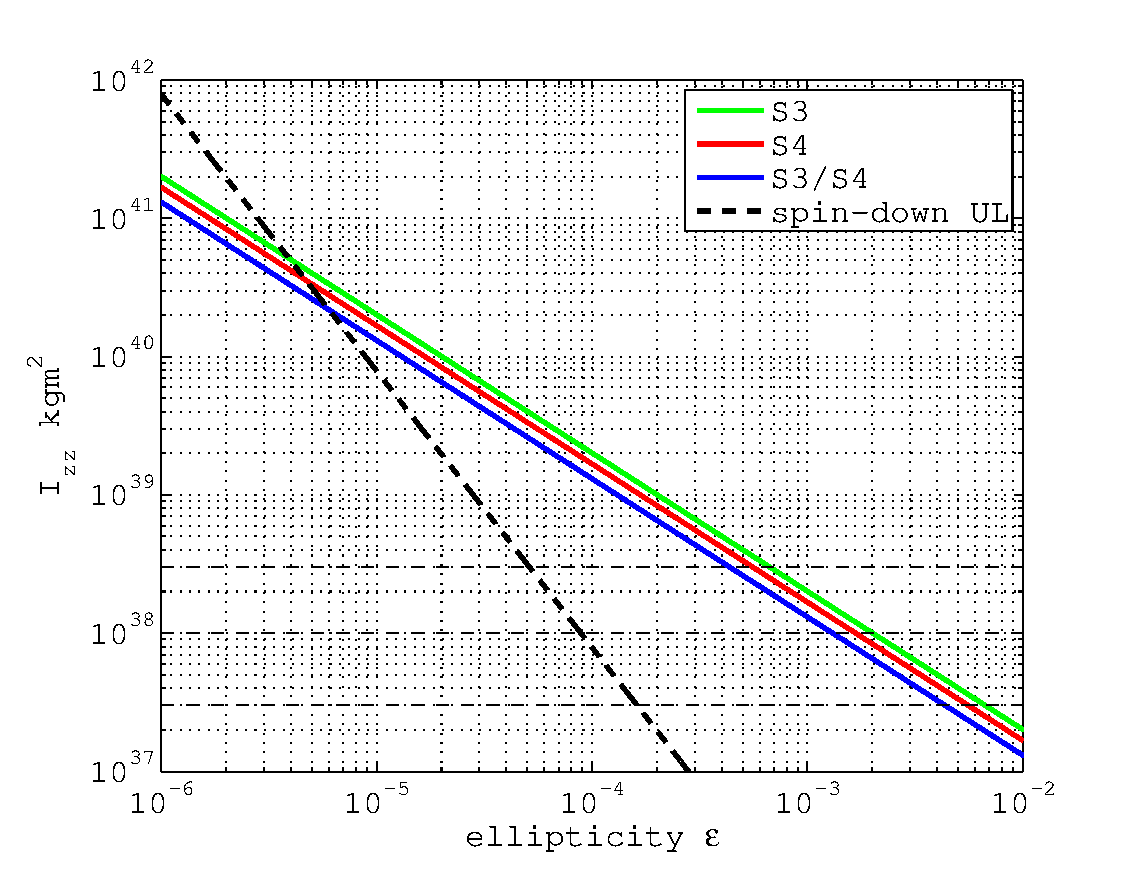
\includegraphics[width=0.6\textwidth]{figs/J0537-6910Ieplane}\caption{The moment of
inertia-ellipticity plane for PSR\,J0537-6910 over the S2, S3 and S4 runs.}\label{J0537-6910Ieplane}
\end{center}
\end{figure}

%In the future it will be well worth checking, with previous authors, for recent observation of this
%pulsar or even attempting our own observing program.

\section{Astrophysical interpretation}\label{astrophysics}
It can be seen from tables~\ref{S3Results}, \ref{S4Results} and \ref{S3S4Results} that for the
majority of pulsars the upper limits we have produced are at least a couple of orders of magnitude
above those from the spin-down argument. If we were to take a pulsar for which our S4 upper limit
was still 100 times above the spin-down limit, we would require an S4 sensitivity run of $\sim 1000$
years until we could match the spin-down limit. This being so is there anything that we can take
from the results in terms of useful astrophysics?

The first thing we can say is that for many of the globular cluster pulsars for which there is a
Doppler induced apparent spin-up we are providing the only limits independent of the pulsars' motion
within the cluster. The maximum apparent spin-up induced by acceleration in a globular cluster is
$4.7\ee{-13}\,{\rm Hz\,s}^{-1}$ for PSR\,J2129+1210D in the cluster M15 \cite{Manchester:2005}. This
large apparent spin-up is due to the pulsar being close to the centre of the cluster and thus being
subject to the largest accelerations. Given this value we can speculate that this is the sort of
magnitude of frequency derivative that could be masked by acceleration effects and therefore use
$-4.7\ee{-13}\,{\rm Hz\,s}^{-1}$ as a maximum {\it spin-down} for all our globular cluster pulsars.
This has not been used here, but may be useful in providing a spin-down upper limit in the future.

It is also interesting to note, despite our limits on the known pulsars being high in relation
to the spin-down ones, that our ellipticity limits are well into the range permitted by at some
models of strange quark stars or hybrid stars ($\varepsilon \sim$ a few times $10^{-4} - 10^{-5}$)
and are reaching into the range permitted by more conventional neutron star EOSs ($\varepsilon \sim$
a few times $10^{-7}$) \cite{Owen:2005}.

Currently the fifth LSC science run (S5) is underway with this providing the possibility of beating
the Crab pulsar spin-down limit within a few months. In reality we will need to be a few times
better than the straight spin-down limit before we can say we are into an interesting regime. This
is because we know that some energy is being lost through magnetic breaking and powering the nebula,
and if we take Palomba's argument stated above we need to be at least 2.5 times better than
spin-down. Again this is assuming our canonical moment of inertia, and some of this may be clawed
back if the Crab pulsar is in the higher mass range. 